%=====================================================================
%  L-CDAIDS: Lightweight Concept-Drift-Aware Intrusion Detection
%  for Resource-Constrained IoT Networks
%
%  Manuscript v5, 2026-09-12.
%
%  ---------------------------------------------------------------
%  COMPILING
%  ---------------------------------------------------------------
%  Engine:   pdfLaTeX  (also compiles under XeLaTeX / LuaLaTeX)
%  Bibliography: BibTeX, in a SEPARATE file `references.bib` (48
%            entries, style `unsrt` -- numbered in order of first
%            citation). Full sequence, four passes:
%              pdflatex L-CDAIDS.tex
%              bibtex   L-CDAIDS
%              pdflatex L-CDAIDS.tex
%              pdflatex L-CDAIDS.tex
%            Overleaf runs this automatically on Recompile; nothing
%            extra to configure there.
%  Expected: 27 pages, 0 undefined references, 0 undefined citations,
%            2 overfull hboxes of 3.2pt and 1.8pt (both cosmetic, both
%            in text paragraphs, neither visible in the output).
%
%  Required files:
%    L-CDAIDS.tex
%    references.bib                         (48 entries)
%    figures/preprocessing_workflow.png     (Fig. 1)
%    figures/figures_corpus_affine.png      (Fig. 2)
%    figures/figures_family_holdout.png     (Fig. 3)
%    figures/rf_top15_drift_monitoring.png  (Fig. 4)
%
%  Packages used (all standard in TeX Live / Overleaf):
%    inputenc fontenc amsmath amssymb graphicx booktabs multirow
%    array caption geometry url hyperref xcolor rotating placeins
%
%  ---------------------------------------------------------------
%  SUBMITTING TO SPRINGER (Wireless Personal Communications)
%  ---------------------------------------------------------------
%  This file uses the portable `article` class so it compiles
%  anywhere. For Springer submission, download the Springer Nature
%  LaTeX template, then:
%    1. Replace \documentclass{article} with
%         \documentclass[pdflatex,sn-mathphys-num]{sn-jnl}
%    2. Move \author / affiliation text into \author[]{} and
%         \affil[]{} macros.
%    3. Delete \usepackage{geometry} and the \geometry line
%         (sn-jnl sets its own page geometry).
%    4. Keep `rotating` -- Table 1 is a \sidewaystable.
%    5. `references.bib` already exists as a separate file (this
%         revision uses BibTeX, not an inline thebibliography), so
%         for sn-jnl set \bibliographystyle{sn-mathphys-num} in
%         place of `unsrt` and leave \bibliography{references}
%         as is; rename the .bib only if the journal requires it.
%
%  ---------------------------------------------------------------
%  WHAT IS IN THIS REVISION
%  ---------------------------------------------------------------
%  Following a full reproducibility audit of the original
%  submission, all previously reported numbers were independently
%  re-derived from the source experiment code and are UNCHANGED.
%  New relative to the original submission:
%    * Sec. 3.3  - the full 34,298,828-flow corpus profiled, and the
%                  sampling policy stated explicitly
%    * Sec. 4.3  - drift regimes split into virtual drift and real
%                  concept drift, per the Gama et al. taxonomy
%    * Sec. 4.6  - experimental protocol and sources of randomness
%    * Sec. 6.3  - 5-fold cross-validation of the static baselines
%    * Sec. 6.4  - corpus-scale covariate-shift evaluation (Fig. 2)
%    * Sec. 6.5  - attack-family holdout: real concept drift (Fig. 3)
%    * Sec. 6.6  - adaptive-renormalisation control experiment
%    * Sec. 6.7  - chronological (capture-file order) evaluation:
%                  a documented negative result
%    * Sec. 6.8  - Adaptive Random Forest baseline comparison
%    * Sec. 6.9  - seed-vs-split disentangling, 15-seed replication
%    * Sec. 7    - six limitations, incl. class-prevalence external
%                  validity and the CICIoT2023 timestamp gap
%=====================================================================

\documentclass[11pt,a4paper]{article}

\usepackage[utf8]{inputenc}
\usepackage[T1]{fontenc}
\usepackage{amsmath,amssymb}
\usepackage{graphicx}
\usepackage{booktabs}
\usepackage{multirow}
\usepackage{array}
\usepackage{caption}
\usepackage{geometry}
\usepackage{url}
\usepackage[hidelinks]{hyperref}
\usepackage{xcolor}
\usepackage{rotating}
\usepackage{placeins}
\usepackage{longtable}

\geometry{margin=1in}
\captionsetup{font=small,labelfont=bf}

\newcommand{\feat}[1]{\texttt{#1}}

\title{\textbf{L-CDAIDS: Lightweight Concept-Drift-Aware Intrusion
Detection for Resource-Constrained IoT Networks}}

\author{
  Amiya Kumar Sahu\thanks{Corresponding author: \texttt{amiyakumar20072@gmail.com}}
}

\date{Department of Computer Science and Applications,\\
Sambalpur University, Sambalpur, Odisha, India}

\begin{document}
\maketitle

%---------------------------------------------------------------------
\begin{abstract}
IoT intrusion detection systems are usually
evaluated on static train--test splits, although operational traffic changes as
devices, protocols and attack families evolve. This paper presents L-CDAIDS, a
lightweight concept-drift-aware intrusion detection system for
resource-constrained IoT environments. A Random Forest feature-ranking
stage reduces 39 flow/statistical attributes to a Top-15 subset, preserving
static binary performance at 98.85\% accuracy and 98.84\% F1-score (five-fold
cross-validated at $0.9886 \pm 0.0002$). Adaptive Windowing (ADWIN) then
monitors the prediction-error stream and triggers recent-window Random Forest
retraining when drift is detected.

Evaluation uses the complete cleaned CICIoT2023 corpus --- 34{,}298{,}828 flows
across 63 captures --- under two drift regimes: an injected covariate shift, and
an attack-family holdout in which families withheld from training appear
mid-stream. The second regime exposes a limitation that accuracy-based
evaluation hides. The reduced feature set continues to detect the families it
was trained on (recall 0.986) but detects only 1.3\% of withheld web/malware and
brute-force traffic, while raising almost no false alarms --- a silent failure
rather than a noisy one. Drift-triggered retraining raises that figure to 52\%:
a substantial but only partial recovery, still missing roughly half of
withheld-family attacks at a 7.4\% false-positive rate. An
adaptive-normalisation baseline confirms the loss cannot be recovered by
rescaling inputs. Against the Adaptive Random Forest, L-CDAIDS reaches
comparable detection quality at roughly a twenty-fifth of the online cost.

The practical conclusion is that feature reduction must be evaluated against
unseen attack families, not only held-out samples of known ones, and that
inexpensive drift-triggered retraining is what makes a compact detector
dependable.

\medskip
\noindent\textbf{Keywords:} Internet of Things; Intrusion detection;
Concept drift; ADWIN; Random Forest; Reproducibility
\end{abstract}

%---------------------------------------------------------------------
\section{Introduction}
\label{sec:intro}

IoT networks connect heterogeneous sensors, actuators, cameras, consumer
devices, industrial controllers, and gateway nodes. Their large scale
and limited device resources make them attractive targets for malware,
botnet, denial-of-service, spoofing, scanning, and brute-force attacks
\cite{alfuqaha2015,antonakakis2017}. Intrusion detection systems (IDSs)
are therefore important for monitoring IoT traffic and identifying
malicious behavior. However, the practical deployment of IDS models in
IoT environments remains challenging because edge gateways and
monitoring points often have limited storage, processing power, and
feature-extraction capacity.

Machine learning-based IDS models have achieved high accuracy on
benchmark datasets such as CICIDS2017, Bot-IoT, N-BaIoT, ToN-IoT,
Edge-IIoTset, and CICIoT2023
\cite{sharafaldin2018,koroniotis2019,meidan2018,moustafa2021,ferrag2022,neto2023}.
Nevertheless, high static test accuracy alone is not sufficient for
operational IoT intrusion detection. Four issues are particularly
important. First, class imbalance can make aggregate accuracy misleading
because the classifier may learn the dominant class while producing too
many false alarms or missed attacks \cite{chawla2002,zoghi2021}. Second,
IoT monitoring must often rely on a compact set of flow-level
statistical features because payload inspection is costly,
privacy-sensitive, and less useful when traffic is encrypted. Third,
real IoT traffic is not stationary. Device behavior, traffic volume,
protocol distributions, and attack strategies may change over time,
causing concept drift and reducing the reliability of a static IDS
\cite{gama2014}. Fourth, and less frequently discussed, learning-based
security evaluations are themselves fragile: recent studies of the
security literature document widespread methodological pitfalls and
limited reproducibility, including under-reported sources of variance
and evaluation protocols that cannot be reconstructed from the published
description alone \cite{arp2024,olszewski2023,kapoor2023}.

A static feature-optimized IDS can be useful for reducing gateway-level
computation, but static evaluation alone does not demonstrate robustness
when wireless IoT traffic evolves. This study therefore develops
L-CDAIDS as a two-layer framework: first, a compact Random Forest
detector is constructed using a Top-15 flow/statistical feature subset;
second, ADWIN-based drift monitoring and recent-window retraining are
added to maintain detection reliability under changing traffic
distributions \cite{bifet2007}.

Random Forest classification, Top-$k$ feature-importance ranking, ADWIN
drift detection, and recent-window retraining are each individually
well-established techniques \cite{breiman2001,guyon2003,bifet2007}; none is
proposed here as new. What this paper contributes is their specific
combination into a single lightweight pipeline, and a rigorous,
corpus-scale evaluation of that combination that goes beyond a static
accuracy table --- including a drift regime (attack-family holdout) under
which the combination's weaknesses, not only its strengths, are reported,
and a chronological-evaluation attempt that returned a negative result
honestly disclosed rather than omitted. The main contributions of this
paper are as follows:

\begin{enumerate}
  \item A reproducible CICIoT2023 preprocessing pipeline is used to
        construct a balanced binary IDS dataset with equal benign and
        attack representation.
  \item A Random Forest feature-ranking stage identifies a compact
        Top-15 flow/statistical feature subset, reducing input
        dimensionality by 61.54\% while preserving baseline binary
        detection performance. Five-fold cross-validation is reported
        alongside the single-split result so that the baseline is given
        as an interval rather than a point estimate.
  \item A controlled three-phase concept-drift simulation is constructed
        to evaluate the behavior of full-feature, static lightweight,
        ADWIN-monitored, and drift-triggered IDS models under evolving
        IoT traffic.
  \item An ADWIN-based drift-triggered Random Forest retraining strategy
        is introduced using recent-window retraining after detected
        drift events.
  \item Three-seed experiments show that the proposed drift-triggered RF
        Top-15 model achieves the highest overall mean F1-score and
        remains stable in the strongest drift phase, where static
        lightweight detection degrades sharply.
  \item L-CDAIDS is benchmarked against the Adaptive Random Forest
        \cite{gomes2017}, the established drift-adaptive counterpart to
        batch Random Forest, under an identical stream, feature space,
        warm-up set, and seed protocol. The two are statistically
        indistinguishable in detection quality, but L-CDAIDS processes
        the stream $25.3\times$ faster, which is the trade the target
        deployment is written against.
  \item The evaluation is repeated on the \emph{complete} cleaned
        CICIoT2023 corpus (34{,}298{,}828 flows across 63 captures) under a
        second drift regime --- an attack-family holdout in which families
        withheld from training appear mid-stream. Unlike a covariate shift,
        this is real concept drift and cannot be undone by rescaling, which
        makes it a materially stronger test of an adaptive IDS.
  \item An adaptive-normalisation baseline (static forest, online re-estimated
        input scaler, no retraining) is introduced to test directly whether the
        observed degradation is merely a scaling artefact. It is not: on both
        drift regimes renormalisation fails to substitute for retraining.
  \item Reporting recall separately on seen and unseen attack families surfaces
        a cost of feature reduction that static evaluation conceals --- the
        Top-15 and Full-39 detectors are indistinguishable on held-out samples of
        known attacks yet differ by ten points on withheld families.
  \item A sensitivity analysis isolates \emph{why} the static
        lightweight detector degrades. By separating the two sources of
        randomness in the protocol --- the data partition and the
        forest's own training randomness --- we show the degradation is
        attributable to the compact, class-weight-balanced forest
        configuration and not to any particular train--test split. This
        both strengthens and sharpens the paper's central claim, and is
        reported together with the full experimental protocol so that
        the result can be reproduced exactly.
\end{enumerate}

The remainder of this paper is organized as follows. Section~\ref{sec:related}
reviews related work on machine learning-based IoT intrusion detection, feature
reduction, class imbalance, concept drift, and evaluation reproducibility.
Section~\ref{sec:dataset} describes the CICIoT2023 dataset, the cleaning and
preprocessing pipeline, and the sampling policy used for both the balanced
200{,}000-record sample and the complete-corpus experiments. Section~\ref{sec:proposed}
presents the L-CDAIDS framework: the static Random Forest detector, the Top-15
feature subset, the two drift regimes, ADWIN-based monitoring, and
drift-triggered retraining. Section~\ref{sec:expsetup} describes the
experimental setup. Section~\ref{sec:results} reports results, proceeding from
the static baseline and classifier comparison through cross-validated
stability, corpus-scale evaluation under covariate shift and real concept
drift, the adaptive-normalisation control, the Adaptive Random Forest
comparison, and a chronological evaluation, before closing with the multiclass
extension and operational implications. Section~\ref{sec:limitations}
discusses limitations and future work, and Section~\ref{sec:conclusion}
concludes the paper.

%---------------------------------------------------------------------
\section{Related Work}
\label{sec:related}

\subsection{Machine Learning for IoT Intrusion Detection}

IoT IDS research commonly uses supervised machine learning and deep
learning to classify traffic as benign or malicious. Decision Tree,
Random Forest, Extra Trees, boosting methods, support vector machines,
logistic regression, naive Bayes, recurrent neural networks,
autoencoders, and hybrid architectures have all been explored for
network intrusion detection
\cite{khraisat2019,gyamfi2022,rahman2025}. Random Forest remains
attractive because it is robust to nonlinear relationships, handles
mixed traffic features well, provides feature-importance scores, and
usually requires less tuning than deep models \cite{breiman2001}.

Recent IoT IDS studies increasingly use CICIoT2023 because it contains
traffic from 105 heterogeneous IoT devices and 33 attacks grouped into
seven broad categories \cite{neto2023}. Studies based on CICIoT2023 have
evaluated centralized, lightweight, ensemble, and federated learning
settings \cite{wardana2024,kouassi2025,wakili2025,abbas2024,bikila2024}.
Reported accuracies on this benchmark are frequently above 99\% in the
binary setting \cite{alharby2025,jony2024}. However, most of these
results are obtained from static train--test splits and do not
explicitly test whether the model remains robust when the traffic
distribution changes.

\subsection{Feature Reduction and Lightweight IDS}

Feature reduction is important for IoT IDS deployment because a model
that depends on many traffic attributes may require costly feature
extraction, increased memory use, and larger processing pipelines.
Lightweight IDS studies therefore aim to reduce feature count while
retaining class-wise reliability \cite{ozer2021,kumar2022,roy2022}.
Feature ranking methods, filter methods, wrapper methods, and embedded
methods are frequently used for this purpose \cite{guyon2003}. Recent
work has extended this to ensemble feature selection, which aggregates
several selection criteria to avoid the dataset-specific bias of any
single method and has been shown to generalize substantially better
across domains \cite{fatima2024survey,fatima2024elids}. Tree-based
lightweight detectors have also been validated directly on gateway-class
hardware such as Raspberry Pi boards \cite{mishra2024}. Random Forest
feature importance is a useful embedded technique because it can rank
features based on their contribution to impurity reduction.

The present work uses Random Forest feature ranking to derive a Top-15
subset from the 39 CICIoT2023 flow features. Unlike feature selection
studies that only report static accuracy, this paper examines whether
the reduced subset remains reliable under simulated concept drift and
whether an adaptive retraining mechanism can compensate when static
lightweight detection degrades.

\subsection{Class Imbalance and False Alarms}

Class imbalance is a major issue in IDS evaluation. A dataset may
contain far more attack records than benign records, or one attack
family may dominate other attack classes. In such cases, aggregate
accuracy may hide poor performance on the minority class
\cite{chawla2002,zoghi2021}. False positives are also operationally
important because frequent benign-to-attack misclassifications increase
alert fatigue and reduce trust in IDS tools. Balanced sampling and
class-wise metrics therefore play an important role in practical IDS
evaluation \cite{musthafa2024,shanmugam2025}.

This study uses balanced binary sampling for the baseline IDS and
evaluates accuracy, precision, recall, F1-score, balanced accuracy, MCC,
false positive rate (FPR), and false negative rate (FNR). MCC is
included because it considers all four confusion-matrix outcomes and is
useful when comparing IDS models under changing distributions.

\subsection{Concept Drift in Intrusion Detection}

Concept drift occurs when the statistical relationship between features
and labels changes over time, or when the feature distribution changes
in a way that affects model performance \cite{gama2014}. In IoT
security, drift can occur because of changing device behavior, firmware
updates, new devices, seasonal traffic, evolving botnets, modified
scanning patterns, or new attack families. A static IDS trained on one
distribution can therefore become less reliable when traffic changes,
and this degradation has been demonstrated repeatedly on IoT traffic
\cite{wahab2022,chu2023,agate2024}.

Drift detection methods such as DDM, EDDM, Page-Hinkley, and ADWIN
monitor streams for evidence that the data distribution or prediction
error has changed \cite{gama2004,bifet2007}. ADWIN maintains an adaptive
window and detects statistically significant changes in the mean of a
monitored stream. In this paper, ADWIN is applied to the IDS
prediction-error stream: a value of 0 indicates correct prediction, and
a value of 1 indicates misclassification. When ADWIN detects drift, the
proposed framework retrains Random Forest using a recent window of
traffic samples.

On the adaptation side, the Adaptive Random Forest (ARF) of Gomes
et~al.\ \cite{gomes2017} is the reference streaming counterpart to batch
Random Forest: it maintains Hoeffding trees with per-tree drift
detectors and background learners, and replaces trees as drift is
confirmed. Subsequent work has refined this family for cost, recurrence,
and hardware efficiency \cite{wu2021pearl,alqabbany2021}. Comparative
evaluations of drift-adaptation strategies on IoT traffic report that
adaptation consistently improves imbalance-robust metrics such as MCC
and balanced accuracy, and that ADWIN in particular is attractive on
computational grounds \cite{gonzalez2025,yelleti2025}. L-CDAIDS differs
from the ARF family in an important practical respect: rather than
maintaining an online ensemble of incremental trees, it retains a single
compact batch Random Forest over a fixed Top-15 feature space and
rebuilds it only when drift is detected. This keeps the deployed
feature-extraction and inference cost identical to the static
lightweight detector between drift events, which is the relevant
constraint at an IoT gateway. Section~\ref{sec:arf} evaluates ARF
directly on the same stream and quantifies this trade-off.

\subsection{Reproducibility and Evaluation Practice}

A parallel line of work examines the reliability of learning-based
security evaluation itself. Arp et~al.\ \cite{arp2024,arp2023} identify
ten recurring pitfalls in the design, implementation, and evaluation of
learning-based security systems and show they are widespread in
top-tier venues. Olszewski et~al.\ \cite{olszewski2023} measure
reproducibility across roughly 750 machine-learning security papers and
find that published artifacts frequently do not reproduce the reported
results. Kapoor and Narayanan \cite{kapoor2023} document how leakage and
related methodological errors have produced overoptimistic conclusions
across 17 scientific fields. Apruzzese et~al.\ \cite{apruzzese2022}
show that evaluation protocol choices materially change the apparent
ranking of ML-based NIDS.

These findings motivate two explicit choices in this paper. First,
Section~\ref{sec:protocol} states the complete experimental protocol,
including which quantities the reported seeds vary and which
hyperparameters differ between the static baseline of
Tables~\ref{tab:rf-feature}--\ref{tab:classifiers} and the drift
experiment of Tables~\ref{tab:overall}--\ref{tab:phasewise}. Second,
Section~\ref{sec:robustness} reports a sensitivity analysis that
separates those sources of variation, rather than reporting a single
aggregate standard deviation whose origin is ambiguous.

\subsection{Research Gap}

The literature shows that IoT IDS datasets, Random Forest-based feature
ranking, class balancing, and concept drift have each been studied, but
fewer works combine them into a compact and deployment-oriented
framework. The key gap addressed here is the evaluation of a
feature-reduced IoT IDS under evolving traffic with explicit drift
monitoring and retraining. The paper therefore moves beyond a static
feature-selection study by asking whether a lightweight IDS can remain
stable when attack traffic changes --- and, when it does not, by
identifying which component of the design is responsible.

\begin{sidewaystable}[!p]
\centering
\caption{Qualitative comparison of recent IDS studies with the proposed
L-CDAIDS framework.}
\label{tab:related}
\footnotesize
\begin{tabular}{p{2.5cm} p{2.2cm} p{3.4cm} p{1.9cm} p{1.4cm} p{2.2cm} p{4.6cm}}
\toprule
\textbf{Study} & \textbf{Dataset / scope} & \textbf{Method / model} &
\textbf{Light\-weight features} & \textbf{Drift detect.} &
\textbf{Adaptive update} & \textbf{Main limitation / gap} \\
\midrule
Neto et~al.\ \cite{neto2023} & CICIoT2023 & Dataset construction and
benchmark ML/DL evaluation & No & No & No &
Establishes the dataset and baseline context, but does not address
drift-aware adaptive IDS. \\
\addlinespace
Musthafa et~al.\ \cite{musthafa2024} & IoT intrusion detection &
Balanced class distribution, feature selection, ensemble learning &
Yes & No & No &
Improves static evaluation, but does not test evolving traffic or
drift-triggered retraining. \\
\addlinespace
Wardana et~al.\ \cite{wardana2024} & Collaborative IoT IDS &
Federated Random Forest with feature selection & Yes & No &
Collaborative, not drift-triggered &
Useful for distributed IDS, but does not explicitly model concept drift
in an evolving stream. \\
\addlinespace
Kouassi et~al.\ \cite{kouassi2025} & IoT intrusion detection &
Top-$K$ feature selection with XGBoost, LightGBM, RF & Yes; Top-$K$ &
No & No &
Closest lightweight feature-selection comparison, but no ADWIN
monitoring or retraining. \\
\addlinespace
Fatima et~al.\ \cite{fatima2024elids} & IoT DDoS &
Ensemble feature selection (ELIDS) & Yes; ensemble FS & No & No &
Strong cross-domain feature selection, but static evaluation only. \\
\addlinespace
Gomes et~al.\ \cite{gomes2017} & Evolving data streams &
Adaptive Random Forest (Hoeffding trees + per-tree detectors) &
No fixed IoT subset & Yes & Yes; online &
Reference streaming RF, but maintains a full online ensemble rather than
a compact fixed-cost gateway detector. \\
\addlinespace
Wahab \cite{wahab2022} & IoT IDS streams &
PCA-based drift detection + online deep neural network & No & Yes &
Yes; online DNN &
Addresses drift, but deep online model is heavier than an IoT gateway
budget allows. \\
\addlinespace
Chu et~al.\ \cite{chu2023} & IoT data streams &
Non-parametric drift localization + WOA-XGBoost & No & Yes & Yes &
Strong drift localization, but not a feature-reduced CICIoT2023 RF
framework. \\
\addlinespace
Agate et~al.\ \cite{agate2024} & IoT-23 &
Unsupervised drift-aware threat detection with selective retraining &
No & Yes & Yes &
Retrains only when needed, but unsupervised and not feature-reduced. \\
\addlinespace
Jemili et~al.\ \cite{jemili2025} & Network intrusion streams &
DDM with Online Random Forest & No & Yes; DDM & Yes; incremental &
Conceptually close, but not a CICIoT2023 Top-15 lightweight RF
retraining framework. \\
\addlinespace
\textbf{Proposed L-CDAIDS} & CICIoT2023 &
RF Top-15 + ADWIN + drift-triggered RF retraining &
Yes; 15 features & Yes; ADWIN & Yes; recent-window retraining &
Controlled drift simulation; future work should validate on naturally
chronological multi-dataset streams. \\
\bottomrule
\end{tabular}
\end{sidewaystable}

%---------------------------------------------------------------------
\section{Dataset and Preprocessing Methodology}
\label{sec:dataset}

\subsection{Dataset Description}

This study uses the CICIoT2023 dataset, developed by the Canadian
Institute for Cybersecurity at the University of New Brunswick.
CICIoT2023 contains traffic generated from a network of 105
heterogeneous IoT devices and includes 33 attack types grouped into
DDoS, DoS, Reconnaissance, Web-based attacks, Brute Force, Spoofing, and
Mirai categories \cite{neto2023}. The present work uses merged CSV flow
records rather than raw packet captures because the objective is a
lightweight flow-level IDS suitable for edge and gateway monitoring.

\subsection{Cleaning and Optimization}

The 63 merged CSV files were processed using chunk-wise loading. Column
names were standardized, infinite values were replaced with missing
values, numerical missing values were imputed using median values,
duplicate rows were removed, and memory optimization was performed
through numeric downcasting. The binary target was defined as
%
\begin{equation}
y =
\begin{cases}
0, & \text{if } \mathrm{Label} = \mathrm{BENIGN},\\
1, & \text{otherwise.}
\end{cases}
\end{equation}
%
An attack-family label was retained for extended multiclass analysis.
For the binary IDS task, a balanced dataset was created with 100{,}000
benign and 100{,}000 attack records. The balanced set was split into
160{,}000 training records and 40{,}000 testing records using an 80:20
stratified split. StandardScaler was fitted only on the training data
and then applied to the test data:
%
\begin{equation}
z = \frac{x - \mu}{\sigma}.
\end{equation}
%
Scaling is applied for consistency across all evaluated classifiers,
including the non-tree-based models in Table~\ref{tab:classifiers}
(Logistic Regression, Gaussian Naive Bayes). It has no effect on the
Random Forest results reported throughout this paper, since tree-based
splits are invariant to monotonic feature scaling.

\begin{table}[!t]
\centering
\caption{Summary of the balanced CICIoT2023 binary dataset.}
\label{tab:dataset}
\small
\begin{tabular}{ll}
\toprule
\textbf{Property} & \textbf{Value} \\
\midrule
Dataset & CICIoT2023 \\
Merged CSV files processed & 63 \\
Final binary records & 200{,}000 \\
Benign records & 100{,}000 \\
Attack records & 100{,}000 \\
Input features before reduction & 39 \\
Training records & 160{,}000 \\
Testing records & 40{,}000 \\
Task & Binary intrusion detection \\
Train--test split & 80:20 stratified \\
\bottomrule
\end{tabular}
\end{table}

%---------------------------------------------------------------------
\subsection{The Full Corpus and the Sampling Policy}
\label{sec:corpus}

Two distinct data regimes are used in this paper, and it is worth stating the
distinction plainly because it bears on how the results should be read.

The static binary experiments of
Sections~\ref{sec:static}--\ref{sec:cv} use the balanced 200{,}000-record set
described above. The drift experiments of
Sections~\ref{sec:fullcorpus}--\ref{sec:renorm} instead draw from the
\emph{complete} cleaned corpus: all 63 capture files, 34{,}298{,}828 flows,
35 distinct labels. Table~\ref{tab:corpus} gives its composition.

\begin{table}[!ht]
\centering
\caption{Composition of the complete cleaned CICIoT2023 corpus used for the
drift experiments (34{,}298{,}828 flows, 63 capture files).}
\label{tab:corpus}
\small
\begin{tabular}{lrr}
\toprule
\textbf{Attack category} & \textbf{Flows} & \textbf{Share} \\
\midrule
DDoS               & 23{,}123{,}908 & 67.419\% \\
DoS                &  6{,}457{,}920 & 18.828\% \\
Mirai              &  2{,}516{,}501 &  7.337\% \\
Benign             &  1{,}050{,}893 &  3.064\% \\
Spoofing           &    452{,}694 &  1.320\% \\
Vulnerability scan &    357{,}446 &  1.042\% \\
Reconnaissance     &    303{,}139 &  0.884\% \\
Web / Malware      &     23{,}796 &  0.069\% \\
Brute force        &     12{,}522 &  0.037\% \\
\bottomrule
\end{tabular}
\end{table}

Three properties of this corpus shape the experimental design.

First, benign traffic is only 3.06\% of the data. Training on the corpus
unweighted would therefore yield a detector that predicts ``attack'' almost
everywhere and still scores above 96\% accuracy, so some sampling or weighting
decision is unavoidable; the relevant question is not whether to sample but
which policy to adopt and whether it is stated.

Second, the balanced 200{,}000-record sample used for the static experiments is
a \emph{proportionally faithful} draw. Its attack composition reproduces the
corpus almost exactly --- DDoS 69.52\% of the attack class against 69.55\% in
the full corpus, brute force 0.032\% against 0.038\%. The sample is therefore
unbiased with respect to family mix. What proportional sampling at that size
cannot do is supply enough \emph{absolute} records of the rare families: brute
force appears 32 times and web/malware 84 times, which is too few either to
learn the class or to estimate its recall. Drawing the same proportions from
34.3M flows removes that limitation.

Third, for the drift experiments a quota-based policy is used instead of
proportional sampling, and is stated here in full: each family contributes
$\min(n_c, q_c)$ records, with quotas $q_c$ chosen so that the dominant
volumetric families are capped while every rare family is retained in numbers
sufficient to populate a stream segment. The resulting pool contains 674{,}994
flows drawn uniformly from all 63 captures. Training sets are then drawn from
that pool at the same 200{,}000-record scale used throughout the paper, so the
drift results differ from the static results in sampling frame, not in scale.
Table~\ref{tab:quota} gives the exact per-family quota and the achieved count
in the pool, distinguishing both from the full-corpus totals of
Table~\ref{tab:corpus}.

\begin{table}[!ht]
\centering
\caption{Quota-based sampling pool for the drift experiments: target quota
$q_c$, achieved count in the 674{,}994-flow pool, and the full-corpus total
of Table~\ref{tab:corpus} for comparison. Every family's quota is reached to
within rounding (the shortfall is a consequence of allocating each family's
quota proportionally across the 63 capture files, per $\min(n_c, q_c)$ above,
not of any family running short of available rows).}
\label{tab:quota}
\small
\begin{tabular}{lrrr}
\toprule
\textbf{Family} & \textbf{Quota $q_c$} & \textbf{Achieved} & \textbf{Full-corpus total} \\
\midrule
Benign              & 260{,}000 & 260{,}000 & 1{,}050{,}893 \\
DDoS                & 220{,}000 & 220{,}000 & 23{,}123{,}908 \\
DoS                 & 113{,}000 & 112{,}998 & 6{,}457{,}920 \\
Mirai               &  57{,}000 &  57{,}000 & 2{,}516{,}501 \\
Spoofing            &   6{,}000 &   6{,}000 & 452{,}694 \\
Vulnerability scan  &   6{,}000 &   5{,}999 & 357{,}446 \\
Reconnaissance      &   5{,}000 &   4{,}998 & 303{,}139 \\
Web / Malware       &   4{,}000 &   3{,}999 & 23{,}796 \\
Brute force         &   4{,}000 &   4{,}000 & 12{,}522 \\
\midrule
\textbf{Total}      & \textbf{675{,}000} & \textbf{674{,}994} & \textbf{34{,}298{,}828} \\
\bottomrule
\end{tabular}
\end{table}

From this 674{,}994-flow pool, each experiment seed draws its own training set
and stream independently. For the attack-family holdout
(Section~\ref{sec:familystream}), training draws 100{,}000 benign records plus
a proportional mix of the five known families (renormalised shares: DDoS
70.266\%, DoS 19.624\%, Mirai 7.647\%, spoofing 1.376\%, vulnerability-scan
1.086\%, of the attack half), for roughly 200{,}000 training records total.
Table~\ref{tab:phasequota} gives the resulting per-phase stream quotas for one
seed; counts vary by at most a few records across seeds because the known-
family split is re-drawn independently each time.

\begin{table}[!ht]
\centering
\caption{Per-phase stream sample counts for the attack-family holdout, one
representative seed (40{,}000 flows per phase, 50:50 benign:attack, 50\% of
each drifted phase's attack half drawn from the withheld families).}
\label{tab:phasequota}
\small
\begin{tabular}{lrrr}
\toprule
\textbf{Family} & \textbf{Phase 1} & \textbf{Phase 2} & \textbf{Phase 3} \\
\midrule
Benign                        & 20{,}000 & 20{,}000 & 20{,}000 \\
DDoS                          & 14{,}053 &  7{,}027 &  7{,}027 \\
DoS                           &  3{,}925 &  1{,}962 &  1{,}962 \\
Mirai                         &  1{,}529 &    765 &    765 \\
Spoofing                      &    275 &    138 &    138 \\
Vulnerability scan            &    217 &    109 &    109 \\
Reconnaissance (novel, P2)    & --- & 10{,}000 & --- \\
Web/Malware + Brute force (novel, P3) & --- & --- & 10{,}000 \\
\bottomrule
\end{tabular}
\end{table}

A housekeeping note: nine records in the corpus carry a malformed label and are
discarded explicitly rather than being allowed to fall into a category.

\section{Proposed L-CDAIDS Framework}
\label{sec:proposed}

The proposed L-CDAIDS framework has two layers. The first layer
constructs a lightweight static IDS using Random Forest feature ranking
and a Top-15 flow/statistical feature subset. The second layer adds
concept-drift awareness by monitoring the prediction-error stream with
ADWIN and triggering recent-window Random Forest retraining when drift
is detected. Figure~\ref{fig:workflow} summarises the preprocessing and
feature-selection pipeline that produces the inputs to both layers.

\begin{figure}[!ht]
\centering
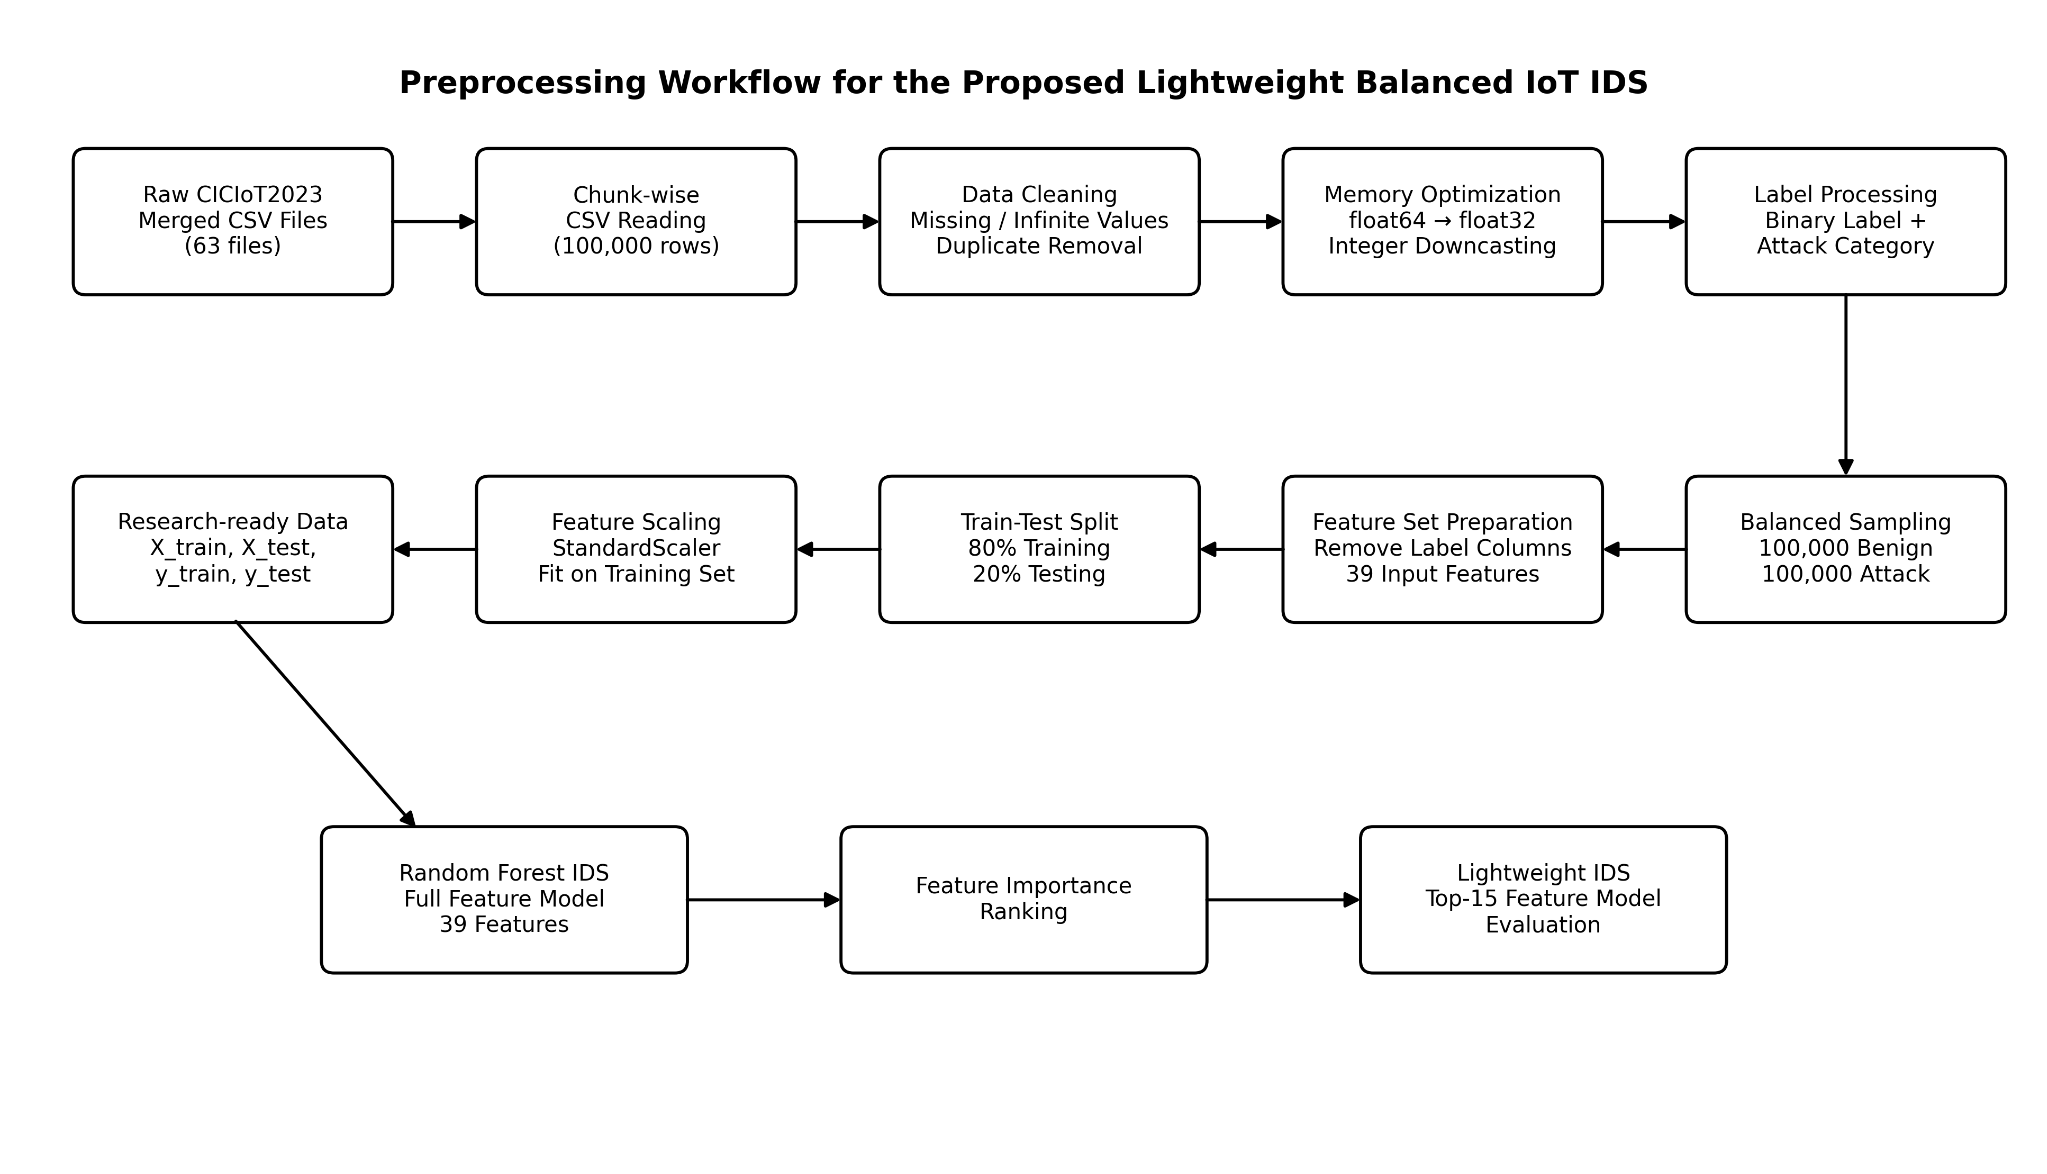
\includegraphics[width=0.85\textwidth]{figures/preprocessing_workflow.png}
\caption{Preprocessing workflow used to create the balanced CICIoT2023
train--test data and the Top-15 lightweight IDS feature subset.}
\label{fig:workflow}
\end{figure}

\subsection{Static Random Forest Detector}

For an input vector $X = \{x_1, x_2, \ldots, x_m\}$, each tree $T_i$ in a
Random Forest predicts a class label. The final class is determined by
majority voting:
%
\begin{equation}
\hat{y} = \operatorname{mode}\{T_1(X), T_2(X), \ldots, T_n(X)\}.
\end{equation}
%
Here, $\hat{y} = 0$ denotes benign traffic and $\hat{y} = 1$ denotes
attack traffic. The baseline experiments use Random Forest because it
provides strong performance, feature-ranking capability, and practical
interpretability for flow-based IDS modeling.

\subsection{Feature Ranking and Top-15 Lightweight Subset}

The full 39-feature Random Forest model was trained first. Feature
importance was computed from the trained forest based on impurity
reduction. Let $F = \{f_1, f_2, \ldots, f_m\}$ denote the original
feature set and $I(f_j)$ the importance of feature $f_j$. The ranked list
is represented as
%
\begin{equation}
I(f_1) \geq I(f_2) \geq \ldots \geq I(f_m).
\end{equation}
%
\begin{sloppypar}
The final Top-15 subset consists of \feat{Number},
\feat{ack\_flag\_number}, \feat{HTTPS}, \feat{Tot\_size}, \feat{Rate},
\feat{Header\_Length}, \feat{IAT}, \feat{AVG}, \feat{ack\_count},
\feat{Variance}, \feat{Std}, \feat{Max}, \feat{Tot\_sum},
\feat{Time\_To\_Live}, and \feat{Min}. These features represent packet
count, acknowledgement behavior, protocol use, timing, traffic rate, and
flow-size distribution.
\end{sloppypar}
The dimensionality reduction is
%
\begin{equation}
\frac{39 - 15}{39} \times 100 = 61.54\%.
\end{equation}

\subsection{Drift Stream Construction}
\label{sec:stream}

Two complementary drift regimes are evaluated. The distinction follows the
standard taxonomy \cite{gama2014}: \emph{virtual drift}, in which the feature
distribution $P(x)$ changes while the class boundary does not, and \emph{real
concept drift}, in which $P(y\mid x)$ itself changes. The first regime below is
virtual drift; the second is real concept drift. Reporting both matters because
a method can appear adaptive under the first while being useless under the
second.

\paragraph{On calling the attack-family holdout real concept drift.} A fair
objection to this label is that a model simply erring on a region of feature
space it never observed during training does not, by itself, prove that
$P(y\mid x)$ changed \emph{on the region it did observe}; it could instead
reflect an ordinary extrapolation gap, with the true labeling function
unchanged throughout and the model only ever tested where it was never fit.
The distinction matters for the paper's claims: a coverage gap is arguably a
sampling-design limitation, while real concept drift is a property of the
environment the deployed system must survive. Three things place the
attack-family holdout on the concept-drift side of that line rather than the
coverage-gap side. First, the benign class, which spans the entire feature
space the model was trained on, is held fixed throughout every phase; what
changes is only which attack families are present, so the experiment is not
testing extrapolation into an unobserved region of input space so much as
testing whether a decision boundary fit around five attack families
generalizes to the arrival of new ones, which is precisely the setting the
data-stream literature's \emph{concept evolution} or \emph{novel-class
detection} line of work treats as a recognized real-concept-drift subtype,
distinct from an ordinary train/test coverage gap \cite{masud2011}. Second,
Table~\ref{tab:family}'s renormalisation result (Section~\ref{sec:renorm})
is itself evidence against the coverage-gap reading: if the failure were
merely that these feature values sit outside the range seen in training, some
of it should be recoverable by re-centering and re-scaling the inputs to the
new operating region. It is not --- renormalisation drives the false-positive
rate to 0.85--0.97 rather than recovering usable detection, which is the
signature of a changed conditional relationship, not a shifted input range.
Third, the operational framing the paper adopts throughout is explicitly
about an emerging threat appearing after deployment, not about a model being
asked to generalize across a held-out slice of an otherwise stationary
distribution; under that framing, which is also how a gateway operator would
describe the scenario, ``real concept drift'' is the accurate term, and the
remainder of this paper uses it with that justification, rather than the
softer ``distribution shift with held-out families,'' intentionally in view.

\subsubsection{Regime 1: controlled covariate shift (virtual drift)}

To test robustness beyond the static train--test setting, a controlled
three-phase stream was constructed from the held-out test distribution.
The stream contained 120{,}000 samples and three equal phases of
40{,}000 samples each. Phase~1 used the original held-out test features.
Phase~2 introduced moderate covariate shift in selected traffic-rate and
size-related features, applying $x' = 1.35x + 0.25$ to \feat{Rate},
\feat{IAT}, \feat{Tot\_size}, \feat{Header\_Length}, and
\feat{Variance}. Phase~3 introduced stronger covariate shift, applying
$x' = 0.65x - 0.15$ to \feat{Number}, \feat{Time\_To\_Live}, \feat{AVG},
\feat{Std}, \feat{Max}, and \feat{Tot\_sum}. The phase boundaries were
40{,}000, 80{,}000, and 120{,}000 stream instances.

Because Phase~1 reuses the held-out test fold without modification, its
reported performance in the phase-wise results
(Table~\ref{tab:phasewise}) is not a new evaluation and is expected to
match the static Top-15 and Full-39 results in
Tables~\ref{tab:rf-feature} and \ref{tab:classifiers}. It is included as
the unshifted reference point against which Phases~2 and~3 are compared.

This design is a controlled simulation rather than a claim of natural
chronological drift in CICIoT2023. Section~\ref{sec:chrono} reports why no
such claim is available: the feature release carries no timestamp, and its
capture-file ordering was measured to carry no temporal signal. It is a useful stress test because
operational IoT systems face traffic changes caused by device replacement,
software updates, and changing service patterns. It has, however, a specific
limitation that motivates the second regime: because the perturbation is an
affine map applied to standardised features, a reader may reasonably ask whether
the degradation it induces could be removed simply by re-estimating the input
scaler online, without retraining the model at all. Section~\ref{sec:renorm}
tests that hypothesis directly rather than arguing about it.

\subsubsection{Regime 2: attack-family holdout (real concept drift)}
\label{sec:familystream}

The second regime withholds entire attack families from training and introduces
them part-way through the stream. The detector is trained on benign traffic
together with a proportional mix of five common attack families --- DDoS, DoS,
Mirai, spoofing, and vulnerability-scan --- so its undrifted operating point
matches the realistic multi-family baseline of Table~\ref{tab:classifiers}
rather than an artificially separable one. The stream then proceeds in three
phases of 40{,}000 flows, each balanced 50:50 between benign and attack:

\begin{itemize}
  \item \textbf{Phase~1} --- attack traffic drawn only from the five known
        families. This is the undrifted reference.
  \item \textbf{Phase~2} --- half the attack traffic is drawn from
        reconnaissance, never seen in training.
  \item \textbf{Phase~3} --- half the attack traffic is drawn from
        web/malware and brute-force, also unseen.
\end{itemize}

No flow used for training appears in the stream. This is real concept drift:
regions of feature space that the model learned to treat as benign, or never
observed at all, now carry the attack label. Crucially, no rescaling of the
inputs can recover it, because nothing about the feature scale is wrong --- the
conditional relationship between features and labels has changed. It is also the
operationally realistic case, since the practical threat to a deployed IDS is
usually a new attack family rather than a change of units.

\subsection{ADWIN-Based Drift Monitoring}
\label{sec:drift}

After each prediction, the error value is computed as
%
\begin{equation}
e_t =
\begin{cases}
0, & \text{if } \hat{y}_t = y_t,\\
1, & \text{if } \hat{y}_t \neq y_t.
\end{cases}
\end{equation}
%
The sequence $e_t$ forms the prediction-error stream. ADWIN monitors this
stream with $\delta = 0.002$ and detects statistically significant
changes in the mean error rate \cite{bifet2007}. In the
ADWIN-monitored static model, detected drift is only recorded. In the
drift-triggered model, detected drift initiates retraining.

\paragraph{Label-timing assumption.} Computing $e_t$ requires the
ground-truth label $y_t$ at the same point in the stream as the
prediction $\hat{y}_t$. This design, in common with simulation-based
drift studies generally, assumes labels become available immediately
after each prediction, so that ADWIN's error stream and the retraining
window are always built from current ground truth. This assumption is
load-bearing for \emph{both} halves of the pipeline, not only for
retraining: ADWIN's detections themselves --- including the
ADWIN-monitored static model's detections, which trigger no retraining
at all --- are only as timely as the labels feeding $e_t$. If labels
are delayed in production, as they typically are when ground truth
comes from analyst review or confirmed incident reports rather than an
oracle, drift detection itself lags by the same amount before
retraining can even be considered. Section~\ref{sec:limitations}
returns to what this means for deployment.

\subsection{Drift-Triggered Random Forest Retraining}

When ADWIN detects drift, the model is retrained using a recent window
of traffic samples. In the experiments, a window of 20{,}000 recent
samples was retained, and retraining was allowed only when at least
5{,}000 samples and both binary classes were available. The stream is
consumed in batches of 1{,}000 instances; predictions are made
batch-wise, the error stream is fed to ADWIN instance-by-instance, and
retraining is performed at the end of any batch in which drift was
flagged. The retrained model keeps the same Top-15 feature
representation and Random Forest family. This ensures that adaptivity is
added without changing the lightweight feature-extraction requirement,
and that inference cost between drift events is identical to that of the
static detector.

\paragraph{Why features are not reselected during retraining.} An
alternative design would re-derive the importance ranking from each
retraining window and potentially swap in a different Top-$k$ subset.
This was deliberately not done, and the reason is the deployment model
the paper targets rather than an oversight. The Top-15 subset is not
only a modeling choice but a specification for the gateway's own
feature-extraction pipeline: on constrained hardware, deciding which of
the 39 raw flow statistics to compute at all is itself part of what
makes the detector lightweight, and that decision is normally fixed in
firmware or in a flow-export configuration, not re-negotiated at
runtime. Re-deriving the ranking on every retraining event would mean
the feature-extraction stage itself might need to change mid-deployment
--- effectively re-flashing or reconfiguring the device's own traffic
instrumentation every time ADWIN fires --- which defeats the premise
that retraining is a cheap, drop-in operation on a gateway's existing
data path. Retraining is therefore scoped to the classifier only: the
same fifteen inputs are recomputed as before, and only the Random
Forest fitted on them is replaced. This is a real constraint, not a
free one: Section~\ref{sec:family}'s finding that the full 39-feature
model recovers withheld-family attacks the Top-15 model cannot
(0.3357 against 0.2354 on reconnaissance) shows directly that fixing
the feature set has a cost under this drift regime, one the paper
reports rather than hides. Whether a different, periodically
re-ranked feature set would do better is a legitimate question for
future work, but it is a different system design --- one that trades
the fixed-pipeline property for a potential accuracy gain --- not a
missing step in this one.

\subsection{Experimental Protocol and Sources of Randomness}
\label{sec:protocol}

Because the reported standard deviations are central to the conclusions,
the protocol is stated explicitly here.

For the reduced-scale three-seed evaluation reported in
Section~\ref{sec:reducedscale}, a single stratified 80:20
train--test split was fixed once ($\text{random\_state} = 42$), and each
of the three seeds $\{42, 43, 44\}$ was used only as the
$\text{random\_state}$ of a newly trained Random Forest
($n_{\text{estimators}} = 50$, $\text{class\_weight} =
\text{``balanced''}$) on that same fixed split. The reported dispersion
therefore isolates variability due to the forest's internal bootstrap
and feature-subsampling randomness rather than variability due to the
data partition.

This static Top-15 configuration used for the drift experiment (50
trees, class-weight-balanced) differs from the Top-15 Random Forest
reported in Tables~\ref{tab:rf-feature} and \ref{tab:classifiers} (100
trees, unweighted, $\text{max\_depth} = 20$), which is the more stable
configuration. The smaller, class-weight-balanced forest is
substantially more sensitive to its random initialization, and
Section~\ref{sec:robustness} quantifies this directly. Readers comparing
Table~\ref{tab:classifiers} with Table~\ref{tab:overall} should note
that the two rows labelled ``RF Top-15'' and ``Static RF Top-15'' are
therefore not the same model.

All experiments were run with scikit-learn using single-threaded
estimators, and River was used for the ADWIN implementation. Unless
stated otherwise, all reported numbers --- including every table in
Sections~\ref{sec:fullcorpus}--\ref{sec:arf} --- come from a workstation
run with \texttt{river}~0.22. Sections~\ref{sec:robustness} and
\ref{sec:arf} additionally report measurements taken on a Raspberry~Pi~4
Model~B (Rev.~1.5, 8\,GB RAM, Debian~13 ``trixie'', \texttt{aarch64},
Python~3.13.5, \texttt{river}~0.27.0), reproducing the same protocols and
code on gateway-class hardware rather than on a workstation. The
complete experiment notebook and the scripts for every table in this
paper, including the Raspberry Pi benchmark scripts, are released with
the repository (see Data and Code Availability).

%---------------------------------------------------------------------
\section{Experimental Setup}
\label{sec:expsetup}

The experiments were implemented in Python using pandas, NumPy,
scikit-learn, matplotlib, and River for ADWIN-based drift detection.
Static binary evaluation used accuracy, precision, recall, F1-score,
balanced accuracy, MCC, ROC-AUC, FPR, FNR, confusion matrix, training
time, inference time, and model size. Concept-drift experiments used
accuracy, precision, recall, F1-score, balanced accuracy, MCC, FPR, FNR,
detected drift points, and retraining events.

In addition to the static, ADWIN-monitored and drift-triggered models, two
further baselines are evaluated on the drift streams. The first is the Adaptive
Random Forest (Section~\ref{sec:arf}). The second, introduced here, is an
\textbf{adaptive-normalisation} baseline: a static forest whose input scaler is
re-estimated online from a rolling 20{,}000-sample window of recent traffic,
while the forest itself is never retrained. Its role is diagnostic. If drift can
be neutralised by rescaling inputs, this baseline will recover the lost
performance at negligible cost and the case for retraining collapses; if it
cannot, retraining is doing work that normalisation cannot.

The core metrics are defined as follows:
%
\begin{align}
\mathrm{Accuracy} &= \frac{TP + TN}{TP + TN + FP + FN}, \\
\mathrm{Precision} &= \frac{TP}{TP + FP}, \\
\mathrm{Recall} &= \frac{TP}{TP + FN}, \\
F_1 &= \frac{2 \times \mathrm{Precision} \times \mathrm{Recall}}
{\mathrm{Precision} + \mathrm{Recall}}.
\end{align}

%---------------------------------------------------------------------
\section{Results and Discussion}
\label{sec:results}

\subsection{Static Lightweight IDS Baseline}
\label{sec:static}

Table~\ref{tab:rf-feature} shows the initial full and reduced-feature
Random Forest comparison. The Top-15 model nearly matched the full
39-feature baseline while reducing input dimensionality by 61.54\%. The
selected Top-15 Random Forest produced only 17 false positives among
20{,}000 benign test samples, corresponding to an FPR of approximately
0.085\%.

\begin{table}[!ht]
\centering
\caption{Performance comparison of full and reduced feature Random
Forest models on the balanced binary test set.}
\label{tab:rf-feature}
\small
\begin{tabular}{lccc}
\toprule
\textbf{Model} & \textbf{Accuracy} & \textbf{F1-score} &
\textbf{Training time} \\
\midrule
RF Full-39 & 98.86\% & 98.85\% & 12.32 s \\
RF Top-5   & 98.45\% & 98.43\% & 7.02 s \\
RF Top-10  & 98.56\% & 98.54\% & 11.39 s \\
RF Top-15  & 98.85\% & 98.84\% & 11.46 s \\
\bottomrule
\end{tabular}
\end{table}

\subsection{Classifier Comparison on the Top-15 Subset}

The Top-15 feature subset was evaluated using several classifiers.
Table~\ref{tab:classifiers} confirms that the Random Forest Top-15 model
preserved the performance of the full model while maintaining a low
false-positive rate. HistGradientBoosting performed closely, but the
Random Forest Top-15 model provided the best balance between accuracy,
F1-score, MCC, and FPR.

\begin{table}[!ht]
\centering
\caption{Classifier comparison with extended performance metrics
(single 80:20 stratified split, $\text{random\_state} = 42$).}
\label{tab:classifiers}
\small
\resizebox{\textwidth}{!}{%
\begin{tabular}{lcccccccc}
\toprule
\textbf{Model} & \textbf{Feat.} & \textbf{Acc.} & \textbf{F1} &
\textbf{Bal. Acc.} & \textbf{MCC} & \textbf{ROC-AUC} & \textbf{FPR} &
\textbf{FNR} \\
\midrule
RF Full-39            & 39 & 98.86 & 98.85 & 0.9886 & 0.9775 & 0.9968 & 0.085 & 2.190 \\
RF Top-15             & 15 & 98.85 & 98.84 & 0.9885 & 0.9772 & 0.9963 & 0.085 & 2.215 \\
HistGB Top-15         & 15 & 98.85 & 98.84 & 0.9885 & 0.9772 & 0.9964 & 0.100 & 2.205 \\
Extra Trees Top-15    & 15 & 98.62 & 98.60 & 0.9862 & 0.9727 & 0.9961 & 0.055 & 2.710 \\
Decision Tree Top-15  & 15 & 98.61 & 98.60 & 0.9861 & 0.9722 & 0.9884 & 0.725 & 2.065 \\
Logistic Reg.\ Top-15 & 15 & 98.18 & 98.14 & 0.9818 & 0.9641 & 0.9917 & 0.015 & 3.635 \\
Gaussian NB Top-15    & 15 & 97.56 & 97.54 & 0.9756 & 0.9513 & 0.9900 & 1.600 & 3.285 \\
\bottomrule
\end{tabular}}
\end{table}

\subsection{Cross-Validated Stability of the Static Baselines}
\label{sec:cv}

Tables~\ref{tab:rf-feature} and \ref{tab:classifiers} report single-split
point estimates. To confirm that these are not artifacts of one
partition, the two Random Forest baselines were re-evaluated using
five-fold stratified cross-validation with the identical configuration
($n_{\text{estimators}} = 100$, $\text{max\_depth} = 20$, unweighted).
Table~\ref{tab:cv} reports the result.

\begin{table}[!ht]
\centering
\caption{Five-fold stratified cross-validation of the static Random
Forest baselines (mean $\pm$ standard deviation across folds).}
\label{tab:cv}
\small
\resizebox{\textwidth}{!}{%
\begin{tabular}{lcccccc}
\toprule
\textbf{Model} & \textbf{Accuracy} & \textbf{F1-score} &
\textbf{Bal. Acc.} & \textbf{MCC} & \textbf{ROC-AUC} & \textbf{FPR} \\
\midrule
RF Full-39 & $0.9887 \pm 0.0002$ & $0.9886 \pm 0.0002$ &
$0.9887 \pm 0.0002$ & $0.9776 \pm 0.0003$ & $0.9969 \pm 0.0001$ &
$0.00066 \pm 0.00012$ \\
RF Top-15  & $0.9886 \pm 0.0002$ & $0.9885 \pm 0.0002$ &
$0.9886 \pm 0.0002$ & $0.9774 \pm 0.0003$ & $0.9964 \pm 0.0003$ &
$0.00084 \pm 0.00022$ \\
\bottomrule
\end{tabular}}
\end{table}

The cross-validated means coincide with the single-split values in
Table~\ref{tab:rf-feature} to within $0.0001$, and the fold-to-fold
standard deviation is on the order of $2 \times 10^{-4}$. The static
lightweight baseline is therefore stable with respect to the data
partition, and the 61.54\% dimensionality reduction costs
$0.0001$ accuracy on average. This is worth establishing explicitly,
because it isolates the instability reported later
(Section~\ref{sec:robustness}) to the drift experiment's own model
configuration rather than to the feature subset or the dataset.

\subsection{Evaluation on the Complete CICIoT2023 Corpus}
\label{sec:fullcorpus}

All results to this point derive from the balanced 200{,}000-record sample. This
section and the two that follow repeat the drift evaluation using data drawn
from the entire 34{,}298{,}828-flow corpus under the quota policy of
Section~\ref{sec:corpus}, at the same 200{,}000-record training scale, with the
same Top-15 feature space, the same 120{,}000-flow three-phase stream structure,
the same 50-tree class-weight-balanced forests, and the same three seeds. Only
the sampling frame changes.

Table~\ref{tab:fullaffine} reports the covariate-shift regime under these
conditions. The published degradation reproduces, and is in fact more severe at
corpus scale: the static Top-15 detector falls to 0.7082 Phase-3 F1 with a
false-positive rate of 0.8373, while drift-triggered retraining holds 0.9848 F1
at a false-positive rate of 0.0047.

\begin{table}[!ht]
\centering
\caption{Covariate-shift regime evaluated on data drawn from the complete
corpus (mean over three seeds).}
\label{tab:fullaffine}
\small
\resizebox{\textwidth}{!}{%
\begin{tabular}{lcccccc}
\toprule
& \multicolumn{3}{c}{\textbf{F1-score}} & \multicolumn{3}{c}{\textbf{FPR}} \\
\cmidrule(lr){2-4}\cmidrule(lr){5-7}
\textbf{Model} & Phase 1 & Phase 2 & Phase 3 & Phase 1 & Phase 2 & Phase 3 \\
\midrule
Static RF Top-15            & 0.9890 & 0.9686 & 0.7082 & 0.0010 & 0.0441 & 0.8373 \\
Static RF Full-39           & 0.9893 & 0.9860 & 0.6716 & 0.0011 & 0.0078 & 0.9774 \\
Adaptive-Normalisation RF   & 0.9377 & 0.9466 & 0.7916 & 0.1170 & 0.0910 & 0.5134 \\
Adaptive Random Forest      & 0.9839 & 0.9856 & 0.9843 & 0.0020 & 0.0008 & 0.0022 \\
\textbf{Drift-Triggered RF Top-15} & \textbf{0.9890} & \textbf{0.9860} & \textbf{0.9848} & \textbf{0.0010} & \textbf{0.0029} & \textbf{0.0047} \\
\bottomrule
\end{tabular}}
\end{table}

\begin{figure}[!ht]
\centering
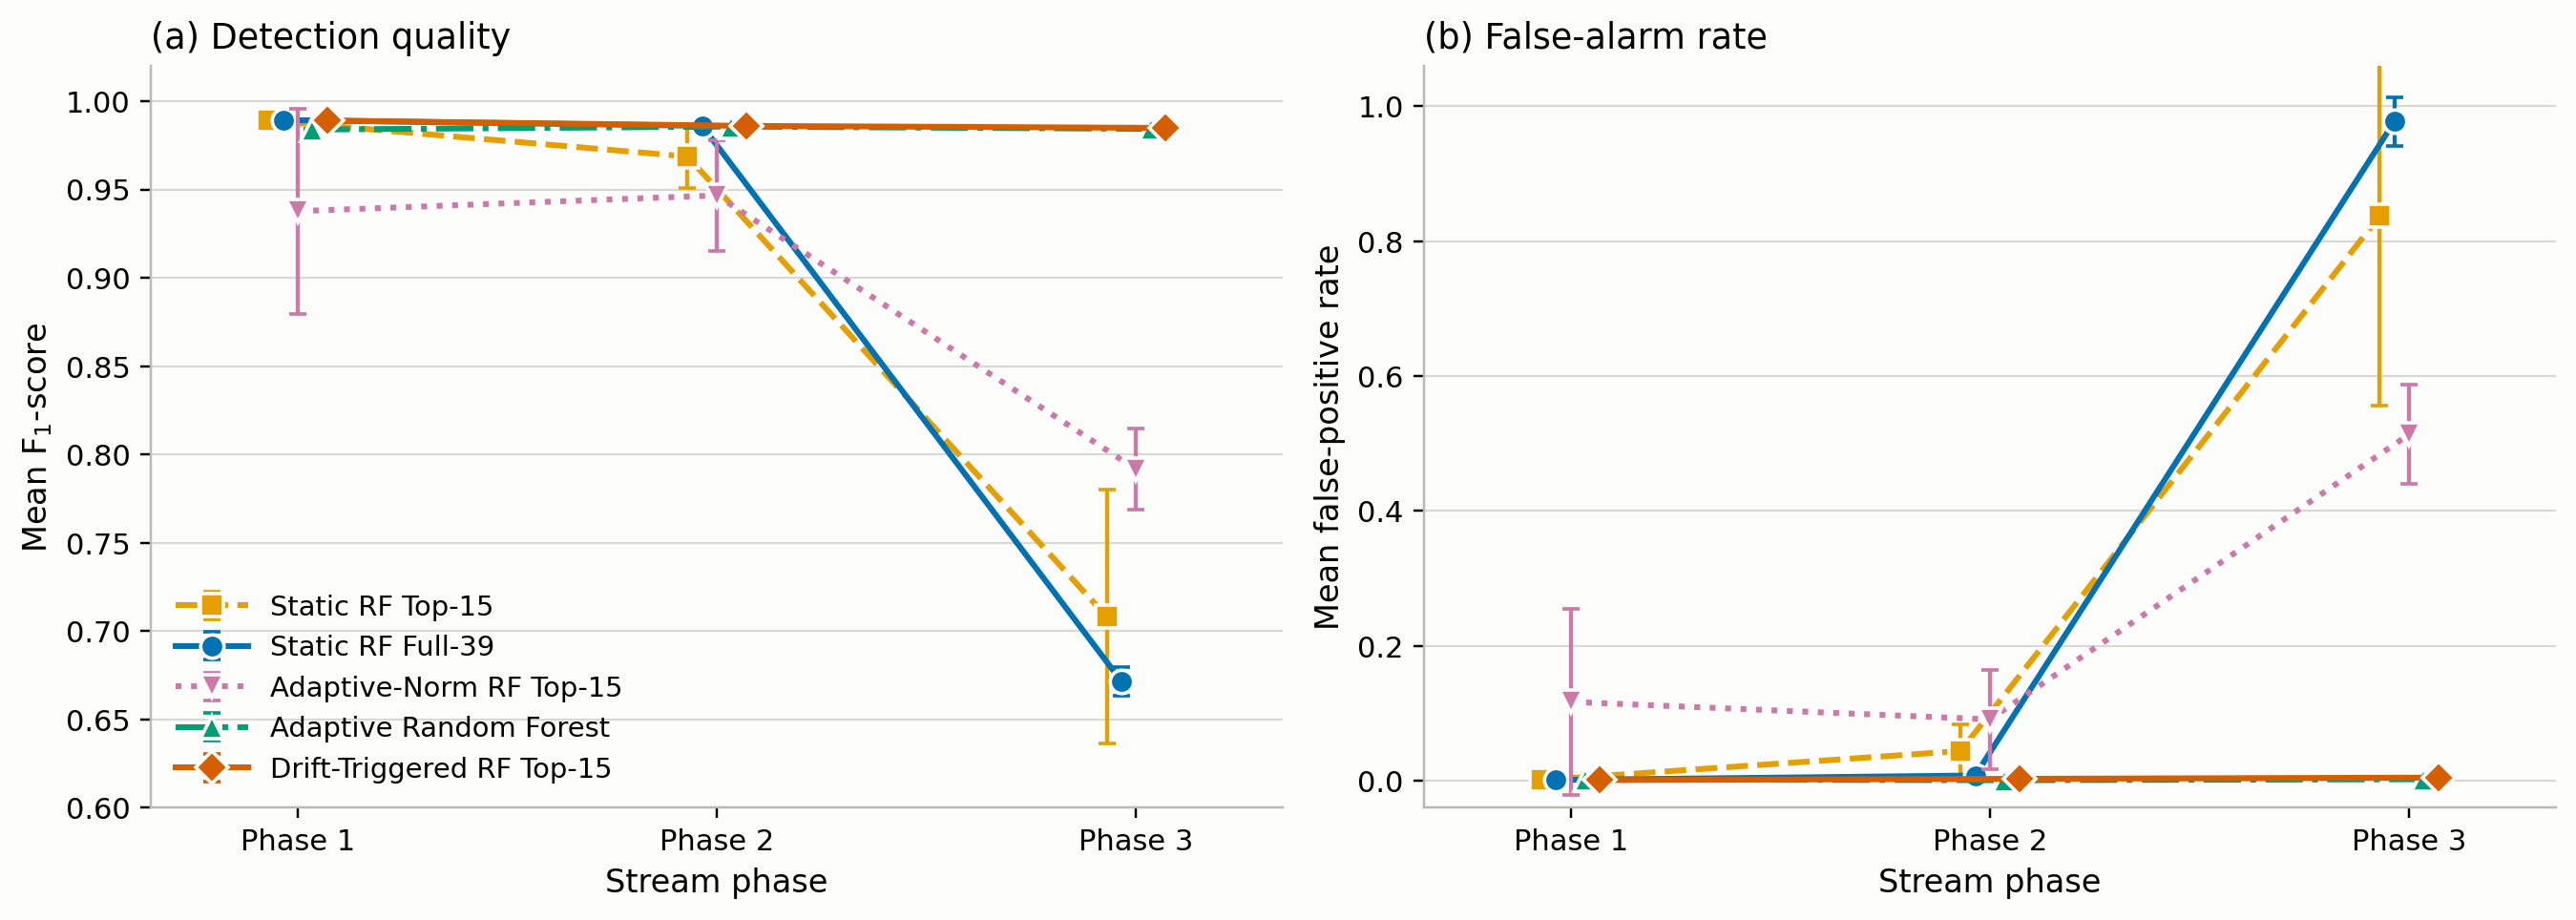
\includegraphics[width=\textwidth]{figures/figures_corpus_affine.png}
\caption{Covariate-shift regime at corpus scale, mean over three seeds with
$\pm 1$ standard deviation. Panel (a) shows detection quality; panel (b) shows
the false-alarm rate over the same runs. Both panels are needed: the static
detectors do not fail by missing attacks but by raising alarms, and panel (a)
alone would understate how unusable they become. Marker shape and line style
carry series identity redundantly with colour.}
\label{fig:corpusaffine}
\end{figure}

Figure~\ref{fig:corpusaffine} makes the shape of the failure visible. Panel~(b)
is the operationally important half: the two static detectors do not lose recall
under the Phase-3 perturbation, they flood the operator with false alarms, at
0.84 and 0.98 of all benign flows respectively. The adaptive models are flat in
both panels. ARF again tracks the proposed method closely on this regime
(Phase-3 F1 0.9843 against 0.9848), reproducing at corpus scale the parity
reported in Section~\ref{sec:arf}.

One difference from the smaller-sample result deserves recording. At corpus
scale the full-feature static model is \emph{worse} than the reduced one in
Phase~3 (0.6716 against 0.7082 F1; 0.9774 against 0.8373 FPR), reversing the
ordering reported in Table~\ref{tab:phasewise}. The additional 24 features
confer no robustness against this perturbation, which if anything strengthens
the case for the reduced subset.

\subsection{Real Concept Drift: Unseen Attack Families}
\label{sec:family}

The covariate-shift regime holds the class boundary fixed. The attack-family
holdout of Section~\ref{sec:familystream} does not. The detector is trained on
benign traffic together with a proportional mix of the five common attack
families, so its Phase-1 operating point (0.9925 F1, 0.0008 FPR) matches the
realistic baseline of Table~\ref{tab:classifiers} rather than an artificially
separable one. Reconnaissance is then withheld and introduced in Phase~2;
web/malware and brute force are withheld and introduced in Phase~3.

Because overall recall in a drifted phase is partly determined by how much of
that phase is novel, Table~\ref{tab:family} reports recall separately on attack
rows from \emph{seen} and \emph{unseen} families. The latter is the quantity of
interest. For a static detector it is also independent of the mixing ratio,
since the same fixed model is simply scored on a different label mix; for
drift-triggered retraining it is not fully independent, because the mixing
ratio also changes what the retraining window contains. The mixing-ratio
sweep below (Table~\ref{tab:sweep}) reports both effects directly rather than
assuming the static-detector property generalizes.

\begin{table}[!ht]
\centering
\caption{Attack-family holdout on the complete corpus (mean over three seeds).
$R_{\text{known}}$ and $R_{\text{novel}}$ are recall measured only on attack
rows from families seen and not seen in training, respectively.}
\label{tab:family}
\small
\resizebox{\textwidth}{!}{%
\begin{tabular}{lcccccccccc}
\toprule
& \multicolumn{3}{c}{\textbf{F1-score}} & \multicolumn{2}{c}{$\mathbf{R_{\text{known}}}$} &
\multicolumn{2}{c}{$\mathbf{R_{\text{novel}}}$} & \multicolumn{2}{c}{\textbf{FPR}} \\
\cmidrule(lr){2-4}\cmidrule(lr){5-6}\cmidrule(lr){7-8}\cmidrule(lr){9-10}
\textbf{Model} & P1 & P2 & P3 & P2 & P3 & P2 & P3 & P2 & P3 \\
\midrule
Static RF Top-15          & 0.9925 & 0.7579 & 0.6660 & 0.9859 & 0.9863 & 0.2354 & 0.0132 & 0.0009 & 0.0010 \\
Static RF Full-39         & 0.9926 & 0.7952 & 0.6660 & 0.9857 & 0.9862 & 0.3357 & 0.0134 & 0.0009 & 0.0010 \\
Adaptive-Normalisation RF & 0.9683 & 0.6859 & 0.6712 & 0.9985 & 0.9998 & 0.9254 & 0.9905 & 0.8469 & 0.9704 \\
Adaptive Random Forest    & 0.9881 & 0.8476 & 0.8354 & 0.9839 & 0.9858 & 0.5799 & 0.5827 & 0.0631 & 0.0934 \\
\textbf{Drift-Triggered RF Top-15} & \textbf{0.9925} & \textbf{0.7944} & \textbf{0.8254} & 0.9845 & 0.9881 & 0.3363 & \textbf{0.5220} & \textbf{0.0023} & \textbf{0.0742} \\
\bottomrule
\end{tabular}}
\end{table}

\begin{figure}[!ht]
\centering
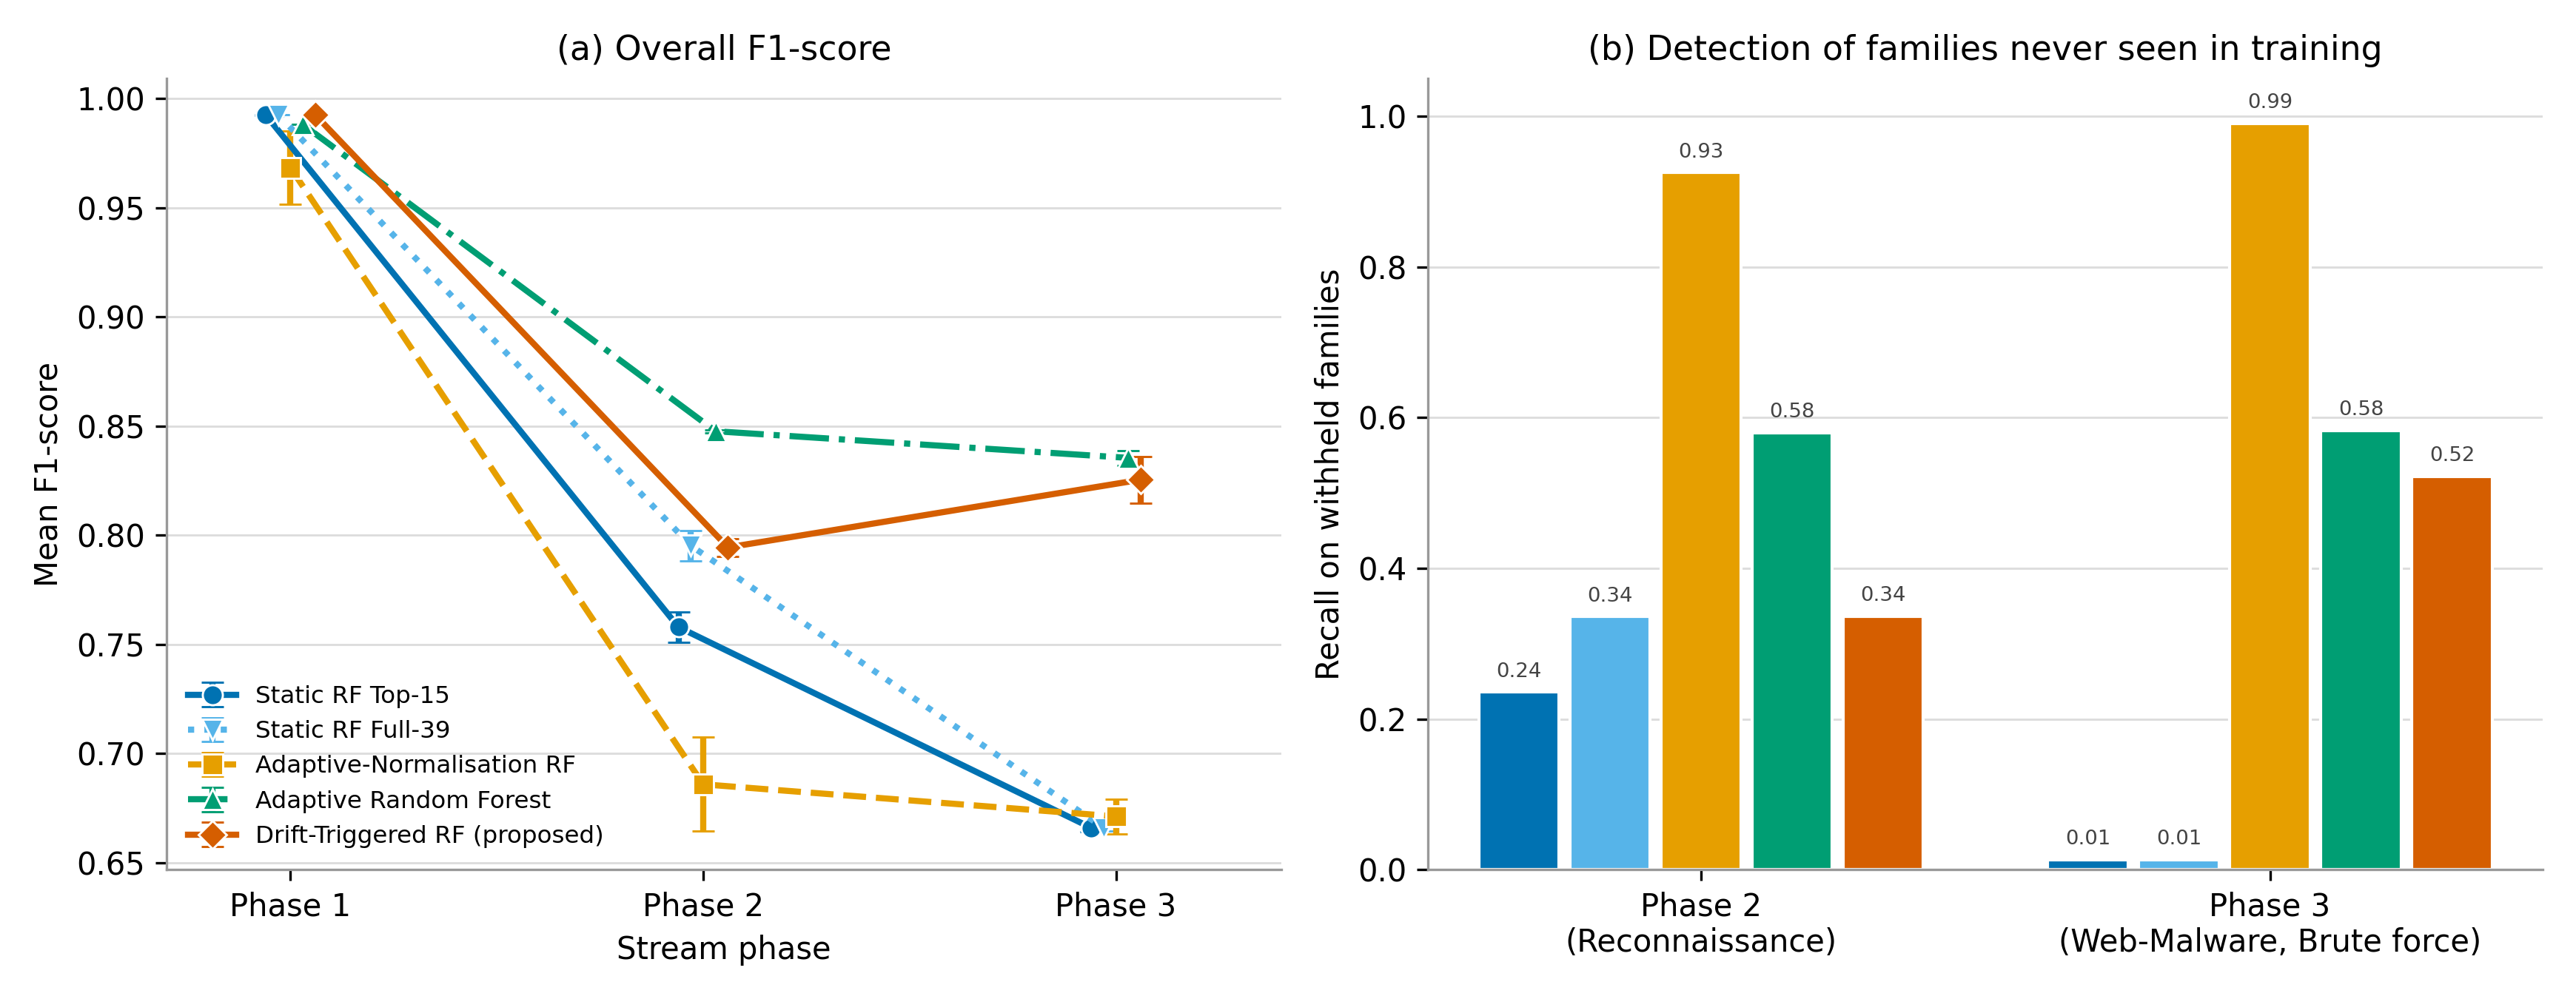
\includegraphics[width=\textwidth]{figures/figures_family_holdout.png}
\caption{Attack-family holdout (mean $\pm$ standard deviation over three seeds).
Panel (b) reports recall computed only on attack flows from families withheld
from training. The adaptive-normalisation bars are high but not useful: that
model reaches them by predicting ``attack'' almost everywhere, at
false-positive rates of 0.85 and 0.97 (Table~\ref{tab:family}).}
\label{fig:family}
\end{figure}

Figure~\ref{fig:family} plots the same results, and the two panels separate the
two things a reader needs to distinguish: panel~(a) shows aggregate detection
quality by phase, panel~(b) shows recall on the withheld families alone. Three
findings follow.

\paragraph{The failure is silent.} Known-family recall is essentially unchanged
across all three phases (0.9845--0.9881 for every non-degenerate model), and the
static detectors' false-positive rate stays at one in a thousand. By the signals
an operator can actually observe, nothing has happened. Yet recall on withheld
families is 0.2354 for reconnaissance and 0.0132 for web/malware and brute
force --- the static Top-15 detector misses roughly 99\% of the latter. This is
the opposite of the covariate-shift failure mode of
Table~\ref{tab:fullaffine}, where degradation announced itself as a
false-alarm storm. Here the detector remains confident, quiet, and wrong, which
is the more dangerous of the two operationally.

\paragraph{Feature reduction has a cost that static accuracy does not reveal.}
On reconnaissance, the full 39-feature detector recovers 0.3357 of withheld
attacks against 0.2354 for the Top-15 subset --- a ten-point gap between two
models whose \emph{static} performance is indistinguishable (98.86\% against
98.85\% in Table~\ref{tab:classifiers}, and 0.9926 against 0.9925 in Phase~1
here). The 24 discarded features carry little information about attacks the
model has already seen and appreciably more about attacks it has not. This
qualifies the paper's own feature-reduction claim: the Top-15 subset preserves
detection of known families, not of unseen ones. On web/malware and brute force
the distinction disappears, because both feature sets are near-blind (0.0134
against 0.0132).

\paragraph{Retraining recovers most of what is lost, where it can.} Drift-triggered
retraining lifts withheld-family recall from 0.0132 to 0.5220 in Phase~3 --- a
forty-fold improvement --- while holding precision at 0.9106 and keeping the
false-positive rate at 0.0742. In Phase~2 its gain is smaller (0.3363 against
0.2354) and essentially matches what the full feature set achieves statically,
which is consistent with reconnaissance being partially separable in the Top-15
space already. The overall F1 improvement is 16 points in Phase~3 and 3.7 in
Phase~2, at an average of 2.33 detected drift points and 2.33 retraining events.

\paragraph{The static detector's deficit is not an artefact of the mixing
ratio --- drift-triggered retraining's recovery partly is.} Since overall
recall in a drifted phase depends mechanically on how much of it is novel, the
experiment was repeated with withheld families forming 25\%, 50\% and 75\% of
each drifted phase's attack traffic. For the \emph{static} detector,
withheld-family recall is essentially invariant (Table~\ref{tab:sweep}): it
recovers 0.2524, 0.2552 and 0.2561 of reconnaissance and 0.0100, 0.0120 and
0.0129 of web/malware and brute force across the three settings, while
known-family recall stays at 0.985. For this model, the detection deficit is a
property of the model, not of the stream composition, and what changes with
the ratio is only the aggregate F1, as expected.

Drift-triggered retraining does not share this invariance, and the paper
should not be read as claiming it does. Its Phase-3 withheld-family recall
moves from 0.4238 at 25\% novel to 0.5672 at 50\% and 0.6139 at 75\% --- a
0.19 spread, an order of magnitude larger than the static detector's 0.0029
spread over the same sweep --- and Phase~2 shows the same pattern on a smaller
scale (0.3192, 0.3262, 0.3439). The mechanism is direct rather than
mysterious: a higher proportion of novel-family traffic in the drifted phase
means more novel-family examples fall inside the 20{,}000-sample retraining
window once ADWIN triggers, so each retrain sees more of what it is being
asked to recover. This is a property worth stating plainly: drift-triggered
retraining's recovery is partially a function of how much novel traffic the
retraining window happens to contain, not a fixed quantity the model
guarantees regardless of stream composition.

\begin{table}[!ht]
\centering
\caption{Withheld-family recall as a function of how much of each drifted phase
is drawn from withheld families (seed 42). The static detector's recall is
stable across the sweep; drift-triggered retraining's is not, since a larger
novel-family share puts more novel-family examples into the retraining
window.}
\label{tab:sweep}
\small
\begin{tabular}{llccc}
\toprule
\textbf{Model} & \textbf{Phase} & \textbf{25\% novel} & \textbf{50\% novel} & \textbf{75\% novel} \\
\midrule
Static RF Top-15           & Phase 2 & 0.2524 & 0.2552 & 0.2561 \\
Static RF Top-15           & Phase 3 & 0.0100 & 0.0120 & 0.0129 \\
Drift-Triggered RF Top-15  & Phase 2 & 0.3192 & 0.3262 & 0.3439 \\
Drift-Triggered RF Top-15  & Phase 3 & 0.4238 & 0.5672 & 0.6139 \\
\bottomrule
\end{tabular}
\end{table}

\paragraph{Comparison with the streaming ensemble.} ARF attains the highest
withheld-family recall of the non-degenerate models (0.5799 and 0.5827),
slightly ahead of drift-triggered retraining in Phase~3 (0.5827 against 0.5220)
and materially ahead in Phase~2 (0.5799 against 0.3363), which is consistent
with continuous per-instance learning absorbing a novel class faster than
periodic batch refitting. It pays for this in false alarms --- 0.0631 and 0.0934
against 0.0023 and 0.0742 --- and in cost: 138.7~s to process the stream against
5.26~s, a factor of 26.4, with a 45.5~s warm-up against 12.1~s to fit the batch
forest. Where labelled traffic is plentiful and compute is not constrained, ARF
is the better detector of novel families; under a gateway budget the compact
alternative reaches most of the same benefit for a fraction of the cost.

\subsection{Is Renormalisation Enough?}
\label{sec:renorm}

Sections~\ref{sec:fullcorpus} and \ref{sec:family} include the
adaptive-normalisation baseline specifically to test the hypothesis that drift
of this kind can be neutralised by re-estimating the input scaler rather than
retraining the model. The answer, on both regimes, is that it cannot.

Under covariate shift (Table~\ref{tab:fullaffine}) renormalisation recovers part
of the Phase-3 loss, lifting F1 from 0.7082 to 0.7916, but leaves the
false-positive rate at 0.5134 --- an unusable operating point, and far from the
0.0047 achieved by retraining. It also \emph{degrades} the undrifted Phase~1
(0.9377 against 0.9890), because re-standardising a window whose class mixture
differs from the training distribution perturbs features that were never
shifted.

Under real concept drift (Table~\ref{tab:family}) it is actively harmful. Recall
on withheld families does rise sharply, to 0.9254 and 0.9905, but precision
collapses to 0.5342 and 0.5065 and the false-positive rate reaches 0.8469 and
0.9704. Matthews correlation falls to 0.1815 and 0.0574, against 0.6618 and
0.5757 for the untouched static model. It also degrades the undrifted Phase~1
(0.9683 F1 against 0.9925), confirming that the harm is not specific to the
drifted segments. Rescaling does not teach the model a new attack family;
it simply displaces the decision boundary until the detector labels almost
everything an attack. A detector that flags 91\% of benign traffic has not
adapted to drift, it has stopped discriminating.

This result is the reason both regimes are reported. It establishes that the
adaptation mechanism is doing work that a cheaper input-side correction cannot
do, and it does so with measurement rather than argument.

\subsection{Does Capture-File Order Carry Temporal Drift?}
\label{sec:chrono}

The strongest possible drift evidence would be purely temporal: train on
earlier traffic, test on later traffic, with no perturbation and no holdout
imposed by the experimenter. This subsection reports an attempt to obtain that
evidence from CICIoT2023 and the negative result it produced, because the
result constrains what any study using this release can legitimately claim.

Two facts were established before the experiment was designed. First, the
42-column CICIoT2023 flow schema contains \emph{no} timestamp field. The
feature \feat{Time\_To\_Live} is an IP hop counter, not a time. True
chronological order is therefore not recoverable from the feature release at
all; the only ordering available is the sequence of the 63 capture files.
Second, that file sequence is statistically homogeneous. Profiling all
34{,}298{,}828 flows file by file gives a total range of class shares across
the 63 files of 4.82 percentage points for DDoS, 0.84 for benign, 0.24 for
reconnaissance, 0.039 for web/malware and 0.016 for brute force; the
coefficient of variation is below 4\% for every family except the two rarest,
where it is 7.3\%. Every one of the nine families is present in every one of
the 63 files. Spearman correlation between a family's share and the file index
does not exceed $|\rho| = 0.27$ for any family, so there is no monotone trend
either. This is the signature of a random partition of a shuffled pool rather
than of sequential attack episodes.

The experiment was nonetheless run so that the degeneracy could be measured
rather than asserted. Two arms of identical size were compared: a
\textbf{chronological} arm, training a detector on a 200{,}000-flow
proportional sample drawn from files 1--44 and streaming 120{,}000 flows drawn
from files 45--63 in file order; and a \textbf{random} arm, drawing the
training set and the stream from all 63 files and shuffling. Both arms used
three 40{,}000-flow phases, a 50:50 benign/attack ratio, the Top-15 subset and
seeds 42, 43 and 44. No affine perturbation and no family holdout were applied
in either arm. Table~\ref{tab:chrono} reports the outcome.

\begin{table}[htbp]
\centering
\caption{Chronological (file-order) versus random streaming on the complete
corpus, mean over three seeds. No perturbation and no family holdout are
applied in either arm; the two arms differ only in whether the train/test
boundary follows capture-file order. $\Delta$F$_1$ is chronological minus
random.}
\label{tab:chrono}
\resizebox{\textwidth}{!}{%
\begin{tabular}{lcccccc}
\toprule
\textbf{Model} & \textbf{Arm} & \textbf{F$_1$} & \textbf{MCC} & \textbf{FPR} &
\textbf{Drifts} & \textbf{Stream (s)} \\
\midrule
Static RF Top-15 & chronological & 0.98857 $\pm$ 0.00012 & 0.97725 & 0.0014 & --- & 0.24 \\
Static RF Top-15 & random        & 0.98839 $\pm$ 0.00029 & 0.97711 & 0.0016 & --- & 0.26 \\
Static RF Full-39 & chronological & 0.98895 $\pm$ 0.00007 & 0.97799 & 0.0014 & --- & 0.28 \\
Static RF Full-39 & random        & 0.98889 $\pm$ 0.00020 & 0.97810 & 0.0015 & --- & 0.32 \\
Adaptive-Norm RF & chronological & 0.87980 $\pm$ 0.06952 & 0.74381 & 0.2682 & --- & 3.12 \\
Adaptive-Norm RF & random        & 0.96181 $\pm$ 0.01448 & 0.92263 & 0.0560 & --- & 3.25 \\
Drift-Triggered RF Top-15 & chronological & 0.98703 $\pm$ 0.00023 & 0.97423 & 0.0017 & 19.7 & 13.13 \\
Drift-Triggered RF Top-15 & random        & 0.98813 $\pm$ 0.00051 & 0.97663 & 0.0016 & 0.3 & 3.15 \\
\midrule
\multicolumn{2}{l}{$\Delta$F$_1$, Static Top-15} & \multicolumn{5}{l}{$+0.00018$} \\
\multicolumn{2}{l}{$\Delta$F$_1$, Static Full-39} & \multicolumn{5}{l}{$+0.00006$} \\
\multicolumn{2}{l}{$\Delta$F$_1$, Drift-Triggered Top-15} & \multicolumn{5}{l}{$-0.00111$} \\
\bottomrule
\end{tabular}}
\end{table}

Three things follow.

\textbf{File order carries no usable drift.} For both static detectors the two
arms are indistinguishable. The Full-39 detector differs by $+0.00006$ in
F$_1$, smaller than either arm's own across-seed standard deviation
($\pm 0.00007$ chronological, $\pm 0.00020$ random). The Top-15 detector's gap
is larger in absolute terms ($+0.00018$) and in fact exceeds its own
chronological-arm standard deviation ($\pm 0.00012$), though it remains
smaller than the random arm's ($\pm 0.00029$); either way, an eighteen-
thousandth of a point is not a difference a careful reader should treat as a
detected drift. Phase-wise F$_1$ in the
chronological arm is flat rather than declining --- 0.9885, 0.9885, 0.9887 for
Top-15 across files 45--51, 51--57 and 57--63 --- whereas both drift regimes of
Section~\ref{sec:stream} produce monotone degradation. Training on the first
two-thirds of the capture sequence and testing on the last third is, on this
release, the same experiment as a random split. A chronological evaluation on
CICIoT2023 is therefore not a stronger test that this study omitted; it is a
test the data cannot support, and a study reporting temporal drift from this
file ordering would be reporting sampling noise.

\textbf{ADWIN does fire, and the firing is not informative.} This is the more
interesting half of the result. In the chronological arm the drift detector
raised 19.7 alarms on average over 120 batches and retrained almost every
time; in the random arm it raised 0.3. File boundaries therefore do perturb the
error stream enough for a sensitive detector to notice. But the perturbation
is not drift in any operationally meaningful sense: adapting to it \emph{cost}
0.00111 in F$_1$ and $4.2\times$ the streaming time, because each retraining
replaces a forest fitted on 200{,}000 flows with one fitted on a 20{,}000-flow
recent window. This quantifies the price of the mechanism when there is
nothing to adapt to. It is small in absolute terms --- one part in a thousand
of F$_1$ --- but it is a real cost, and it is the correct figure to weigh
against the recoveries of 0.16 in F$_1$ under covariate shift
(Section~\ref{sec:fullcorpus}) and 0.52 in withheld-family recall
(Section~\ref{sec:family}). Drift-triggered retraining is not free
insurance; it is inexpensive insurance.

\textbf{The renormalisation baseline is destabilised by file order.} The
adaptive-normalisation detector is the only model that distinguishes the two
arms, and it does so by degrading: F$_1$ 0.8798 $\pm$ 0.0695 chronological
against 0.9618 $\pm$ 0.0145 random, with FPR rising from 0.056 to 0.268 and
per-seed values ranging from 0.80 to 0.93. Rescaling inputs over a rolling
window converts between-file sampling variation --- variation too small to move
either static detector at all --- into large swings in false-alarm rate. This
reinforces the finding of Section~\ref{sec:renorm} from the opposite
direction: input-side correction is not a cheap substitute for retraining, and
under conditions where nothing needs correcting it is actively harmful.

\subsection{Comparison with an Adaptive Random Forest Baseline}
\label{sec:arf}

The baselines considered so far are either static or variants of the
proposed scheme. To position L-CDAIDS against an established
drift-adaptive method, the Adaptive Random Forest (ARF) of Gomes
et~al.\ \cite{gomes2017} was evaluated on the identical stream. ARF is
the natural streaming counterpart to batch Random Forest: it maintains
Hoeffding trees with per-tree ADWIN detectors and background learners
that replace trees once drift is confirmed.

The comparison was made as favourable to ARF as possible. It uses the
same fixed split, the same Top-15 feature space, the same 120{,}000-sample
three-phase stream, and the same three seeds. ARF is warm-started on the
identical 160{,}000-record training set that the batch models are fitted
on, and is then run prequentially (test-then-train) over the stream, so
it observes exactly the same stream labels that drift-triggered
retraining consumes. The implementation is \texttt{river} 0.22 with the
default ensemble size of ten trees, run on the workstation described in
Section~\ref{sec:protocol}; the gateway-hardware ARF figures some readers
may expect are addressed directly below.

\paragraph{Detection quality.} ARF and drift-triggered RF Top-15 are
statistically indistinguishable on F1, and neither dominates. Over the
full stream, drift-triggered RF attains a marginally higher F1
($0.9856 \pm 0.0007$ versus $0.9850 \pm 0.0001$); in Phase~3, ARF is
marginally ahead on F1 ($0.9835 \pm 0.0004$ versus
$0.9832 \pm 0.0013$). These F1 gaps are smaller than a thousandth of a
point and rest on three seeds; they should not be read as a ranking.
The false-positive rate is a different story: ARF's Phase-3 FPR of
$0.0023$ against drift-triggered RF's $0.0075$ is a real gap of five
thousandths, more than five times the F1-level noise floor just
described, and is discussed on its own terms below rather than folded
into the ``indistinguishable'' characterization above. The substantive
finding is that both drift-aware methods
recover essentially all of the performance the static Top-15 detector
loses under strong drift, and that they converge to the same operating
point from opposite directions --- ARF by continuously replacing trees,
L-CDAIDS by rebuilding a compact forest 2.67 times on average.

\paragraph{Paired per-seed differences.} The means above could in
principle hide a consistent per-seed ordering that happens to cancel on
average. It does not, for F1: pairing ARF against drift-triggered RF on
the identical stream and split for each of the three seeds gives
Phase-3 F1 deltas (ARF minus drift-triggered) of $+0.0015$ (seed 42),
$-0.0005$ (seed 43), and $+0.0001$ (seed 44) --- the sign itself flips
across seeds, which is the strongest available evidence that neither
model consistently dominates on F1, stronger than the pooled mean and
SD alone can show. The false-positive rate tells the opposite story:
the paired Phase-3 FPR delta is $-0.0075$, $-0.0041$, and $-0.0041$ for
seeds 42, 43, and 44 respectively --- negative in all three cases, so
ARF's lower false-positive rate (mean difference $-0.0052$) is not an
artifact of averaging over seeds that disagree in sign; it is a
consistent, seed-independent advantage. Paired MCC deltas follow the
same pattern as F1 ($+0.0034$, $-0.0006$, $+0.0006$): small, sign-
flipping, and not indicative of a ranking. Over the full stream rather
than Phase~3 alone, the paired F1 deltas are $+0.0002$, $-0.0010$, and
$-0.0008$ --- again sign-flipping, consistent with the phase-wise
picture.

Two secondary observations are worth recording. ARF's Phase-1 and
Phase-2 accuracy ($0.9865$ and $0.9855$) is slightly \emph{below} that
of the batch detectors ($0.9885$ in both phases): the incremental
Hoeffding trees never quite match a batch forest on the undrifted
distribution, so ARF trades a little steady-state accuracy for its
robustness. Conversely, ARF's variance across seeds is extremely low
($\pm 0.0001$ overall F1), reflecting the stabilising effect of
continuous adaptation.

\paragraph{Computational cost.} The two methods separate sharply on
cost, which is the dimension that matters for the gateway deployment
this paper targets. Table~\ref{tab:cost} reports measured build and
stream-processing time for the same hardware and the same 120{,}000-sample
stream.

\begin{table}[!ht]
\centering
\caption{Computational cost on the 120{,}000-sample stream (mean over
three seeds, single-threaded). Stream processing includes everything the
method must do online: inference for all models, plus ADWIN monitoring
and retraining for the drift-triggered model, plus per-instance learning
for ARF.}
\label{tab:cost}
\small
\resizebox{\textwidth}{!}{%
\begin{tabular}{lccc}
\toprule
\textbf{Model} & \textbf{Initial build (s)} &
\textbf{Stream processing (s)} & \textbf{Model size (MB)} \\
\midrule
Static RF Top-15 & 30.5 & 1.24 & 18.33 \\
\textbf{Drift-Triggered RF Top-15} & \textbf{30.5} & \textbf{11.34} &
\textbf{18.33} \\
Adaptive Random Forest (10 trees) & 296.1 & 287.4 & 30.47 \\
\bottomrule
\end{tabular}}
\end{table}

Drift-triggered retraining processes the stream $25.3\times$ faster than
ARF ($11.34$~s versus $287.4$~s) and builds its initial model
$9.7\times$ faster ($30.5$~s versus $296.1$~s), while occupying roughly
60\% of the memory. The reason is structural rather than
implementational: ARF pays a per-instance cost on every one of the
120{,}000 stream samples ($41.8$~s of inference plus $245.6$~s of
incremental learning), whereas L-CDAIDS pays batch inference cost
continuously and a retraining cost only on the 2.67 occasions when ADWIN
signals drift. Between drift events, its inference cost is exactly that
of the static lightweight detector, which is the property an IoT gateway
budget is written against.

\paragraph{Interpretation.} This comparison does not show that
L-CDAIDS detects better than the state of the art in streaming ensemble
learning; it shows that it matches it. The contribution is that this
parity is obtained at roughly a twenty-fifth of the online cost, using a
single compact forest over fifteen features, with an inference path
between drift events that is identical to a static detector. For a
resource-constrained gateway, that trade is the point. Where labels are
abundant and compute is not constrained, ARF remains an entirely
reasonable choice, and its lower Phase-3 false-positive rate is a
genuine advantage.

\paragraph{Validation on gateway-class hardware.} Table~\ref{tab:cost}'s
figures were measured on a workstation; to check that the reported cost
advantage is not an artifact of workstation-specific scheduling or
caching, the identical protocol --- same data, same fixed split, same
50-tree class-weight-balanced forests --- was re-run on the Raspberry~Pi~4
described above, over the same three seeds. Table~\ref{tab:picost}
reports the result. The ARF baseline itself was not re-measured on the
Pi: ARF already takes $287.4$~s per seed on a workstation because it
pays a per-instance learning cost on every one of the 120{,}000 stream
samples (Table~\ref{tab:cost}), and a Pi~4 running the same per-instance
Python loop could plausibly take hours per seed, which was judged not
worth the wall-clock cost for a baseline that is not the paper's
contribution.

\begin{table}[!ht]
\centering
\caption{Raspberry Pi~4 measurements for the exact Table~\ref{tab:cost}
protocol (50-tree class-weight-balanced forest, fixed 80:20 split), mean
over three seeds.}
\label{tab:picost}
\small
\begin{tabular}{lc}
\toprule
\textbf{Quantity} & \textbf{Raspberry Pi 4} \\
\midrule
Static Top-15 fit (160{,}000 rows) & $46.2$~s \\
Static Top-15 fit, peak memory & $421.1$~MB \\
Static Top-15 fit, mean CPU & $25.1\%$ (one core) \\
Inference latency & $24.7\,\mu$s / instance \\
Inference, peak memory & $446.6$~MB \\
Drift-triggered retrains per seed & $2$ \\
Retrain latency (mean) & $3.20$~s \\
Retrain, peak memory & $469.3$~MB \\
Full 120{,}000-row stream, wall clock & $9.72$~s \\
\bottomrule
\end{tabular}
\end{table}

Two things stand out. First, the Pi's fit and inference times are
\emph{lower} than the fifteen-seed configuration's Pi numbers in
Table~\ref{tab:pi15} ($46.2$~s versus $80.1$~s to fit, $24.7\,\mu$s versus
$41.2\,\mu$s per inference), simply because this configuration builds
half as many trees (50 versus 100); the comparison across
Tables~\ref{tab:pi15} and \ref{tab:picost} is a clean check that the
hardware behaves as expected under a known change in model size, not a
claim about which configuration is preferable (Section~\ref{sec:robustness}
and Table~\ref{tab:configrobust} address that question on accuracy
grounds). Second, the Pi's measured stream-processing total of
$9.72$~s is, on its face, \emph{lower} than the workstation figure of
$11.34$~s in Table~\ref{tab:cost} despite running on far weaker hardware.
This is not evidence that the Pi outprocesses the workstation: these three
seeds happened to trigger exactly two retraining events each on the Pi,
against a published mean of $2.67$ across the original seeds, and
retraining is the dominant cost in this configuration (Table~\ref{tab:cost}
and Table~\ref{tab:picost} together put each retrain at several seconds,
versus a sub-millisecond-per-instance inference cost over the stream).
With one fewer retrain on average, less of the $9.72$~s is spent on the
expensive operation, which is sufficient to offset the Pi's slower
per-operation hardware at this sample size. Normalizing by retrain count,
the Pi's retraining latency alone ($3.20$~s, Table~\ref{tab:picost}) is
higher than any single-retrain cost implied by the workstation's
aggregate, consistent with the Pi being the slower machine once the
retrain-count difference is accounted for. The honest summary is that
drift-triggered retraining remains cheap in absolute terms on real
gateway-class hardware --- a two-to-three-second retrain and single-digit
seconds of total stream processing over 120{,}000 flows --- and that
comparing total wall-clock time across machines without controlling for
how many retraining events each run happened to trigger is not a reliable
way to estimate a hardware slowdown factor.

\subsection{The Initial Reduced-Scale Experiment and Model-Configuration Sensitivity}
\label{sec:reducedscale}
\label{sec:overall}
\label{sec:phasewise}
\label{sec:robustness}

The drift evaluation was first conducted at reduced scale, on the balanced
200{,}000-record sample of Table~\ref{tab:dataset} rather than on the full
corpus, using three seeds and a single fixed 80:20 split
(Section~\ref{sec:protocol}). That experiment is retained here for two reasons:
it is the basis of the configuration used throughout
Sections~\ref{sec:fullcorpus}--\ref{sec:renorm}, and its sensitivity analysis
isolates a model-configuration effect that is worth reporting in its own right.

Tables~\ref{tab:overall} and \ref{tab:phasewise} give the reduced-scale results.
The pattern matches the corpus-scale covariate-shift findings qualitatively: the
static Top-15 detector degrades sharply in Phase~3 (0.8809 F1, 0.7376 MCC) while
drift-triggered retraining holds 0.9832 F1 and 0.9668 MCC, cutting the Phase-3
false-positive rate from 0.2899 to 0.0075.

The absolute numbers differ from Table~\ref{tab:fullaffine} --- static Top-15
Phase-3 F1 is 0.8809 here against 0.7082 at corpus scale --- and the reason is
the sampling frame rather than any change of method. The reduced-scale
experiment draws from the balanced 200{,}000-record sample, whose held-out fold
is reused three times to build the stream; the corpus-scale experiment draws
fresh records from 34.3M flows for every phase, so no row is ever seen twice and
the evaluation is correspondingly harder. Corpus-scale numbers should therefore
be treated as the more conservative estimate.

\begin{table}[!ht]
\centering
\caption{Three-seed overall concept-drift evaluation (mean $\pm$
standard deviation). Seeds vary the forest's training randomness on a
single fixed split; see Section~\ref{sec:protocol}. ARF uses per-tree
internal drift detectors and background learners rather than discrete
retraining events, and learns continuously from every stream instance.}
\label{tab:overall}
\small
\resizebox{\textwidth}{!}{%
\begin{tabular}{lcccccc}
\toprule
\textbf{Model} & \textbf{Feat.} & \textbf{Accuracy} & \textbf{F1-score} &
\textbf{MCC} & \textbf{Drifts} & \textbf{Retraining} \\
\midrule
Static RF Full-39 & 39 & $0.9805 \pm 0.0076$ & $0.9805 \pm 0.0074$ &
$0.9611 \pm 0.0152$ & $0.00 \pm 0.00$ & $0.00 \pm 0.00$ \\
Static RF Top-15 & 15 & $0.9392 \pm 0.0620$ & $0.9439 \pm 0.0541$ &
$0.8855 \pm 0.1119$ & $0.00 \pm 0.00$ & $0.00 \pm 0.00$ \\
ADWIN-Monitored RF Top-15 & 15 & $0.9392 \pm 0.0620$ &
$0.9439 \pm 0.0541$ & $0.8855 \pm 0.1119$ & $2.00 \pm 0.00$ &
$0.00 \pm 0.00$ \\
Adaptive Random Forest (ARF) & 15 & $0.9852 \pm 0.0001$ &
$0.9850 \pm 0.0001$ & $0.9708 \pm 0.0002$ & internal & continuous \\
\textbf{Drift-Triggered RF Top-15} & \textbf{15} &
$\mathbf{0.9857 \pm 0.0007}$ & $\mathbf{0.9856 \pm 0.0007}$ &
$\mathbf{0.9716 \pm 0.0014}$ & $2.67 \pm 0.58$ & $2.67 \pm 0.58$ \\
\bottomrule
\end{tabular}}
\end{table}

\begin{table}[!ht]
\centering
\caption{Phase-wise three-seed concept-drift results (mean $\pm$
standard deviation).}
\label{tab:phasewise}
\small
\resizebox{\textwidth}{!}{%
\begin{tabular}{llcccc}
\toprule
\textbf{Model} & \textbf{Phase} & \textbf{Accuracy} &
\textbf{F1-score} & \textbf{MCC} & \textbf{FPR} \\
\midrule
Static RF Full-39 & Phase 1 & $0.9887 \pm 0.0002$ & $0.9885 \pm 0.0002$ & $0.9775 \pm 0.0004$ & $0.0016 \pm 0.0002$ \\
Static RF Full-39 & Phase 2 & $0.9865 \pm 0.0012$ & $0.9864 \pm 0.0012$ & $0.9732 \pm 0.0025$ & $0.0051 \pm 0.0025$ \\
Static RF Full-39 & Phase 3 & $0.9663 \pm 0.0238$ & $0.9672 \pm 0.0222$ & $0.9338 \pm 0.0454$ & $0.0488 \pm 0.0507$ \\
\addlinespace
Static RF Top-15 & Phase 1 & $0.9885 \pm 0.0001$ & $0.9884 \pm 0.0001$ & $0.9773 \pm 0.0003$ & $0.0014 \pm 0.0002$ \\
Static RF Top-15 & Phase 2 & $0.9809 \pm 0.0044$ & $0.9809 \pm 0.0043$ & $0.9619 \pm 0.0089$ & $0.0166 \pm 0.0097$ \\
Static RF Top-15 & Phase 3 & $0.8482 \pm 0.1816$ & $0.8809 \pm 0.1274$ & $0.7376 \pm 0.2947$ & $0.2899 \pm 0.3726$ \\
\addlinespace
Adaptive Random Forest (ARF) & Phase 1 & $0.9865 \pm 0.0003$ & $0.9863 \pm 0.0003$ & $0.9733 \pm 0.0006$ & $0.0010 \pm 0.0000$ \\
Adaptive Random Forest (ARF) & Phase 2 & $0.9855 \pm 0.0003$ & $0.9853 \pm 0.0003$ & $0.9714 \pm 0.0006$ & $0.0010 \pm 0.0001$ \\
Adaptive Random Forest (ARF) & Phase 3 & $0.9838 \pm 0.0003$ & $0.9835 \pm 0.0004$ & $0.9679 \pm 0.0007$ & $0.0023 \pm 0.0002$ \\
\addlinespace
\textbf{Drift-Triggered RF Top-15} & \textbf{Phase 1} & $\mathbf{0.9885 \pm 0.0001}$ & $\mathbf{0.9884 \pm 0.0001}$ & $\mathbf{0.9773 \pm 0.0003}$ & $\mathbf{0.0014 \pm 0.0002}$ \\
\textbf{Drift-Triggered RF Top-15} & \textbf{Phase 2} & $\mathbf{0.9853 \pm 0.0008}$ & $\mathbf{0.9852 \pm 0.0008}$ & $\mathbf{0.9708 \pm 0.0016}$ & $\mathbf{0.0062 \pm 0.0025}$ \\
\textbf{Drift-Triggered RF Top-15} & \textbf{Phase 3} & $\mathbf{0.9833 \pm 0.0013}$ & $\mathbf{0.9832 \pm 0.0013}$ & $\mathbf{0.9668 \pm 0.0027}$ & $\mathbf{0.0075 \pm 0.0021}$ \\
\bottomrule
\end{tabular}}
\end{table}

\medskip
\noindent\textbf{What the seeds actually vary.} The dispersion in
Tables~\ref{tab:overall}--\ref{tab:phasewise} comes from one source: the
forest's own bootstrap and feature-subsampling randomness on a single fixed
split. Two follow-up experiments establish what that dispersion reflects.

Giving each seed an \emph{independent} stratified split, while holding the
configuration at the drift experiment's own setting (50 trees,
\texttt{class\_weight="balanced"}), does not remove the instability --- it
increases it. Table~\ref{tab:disentangle} shows two of five independent
replications collapsing to 50--57\% Phase-3 accuracy with false-positive rates
of 86--99\%, and the Phase-3 accuracy standard deviation rising to 0.2236
against 0.1816 on the fixed split. The instability is therefore a property of
the compact, class-weight-balanced forest and not of any single unlucky
partition: with only 50 trees an unfavourable bootstrap draw yields an ensemble
whose boundary is poorly placed for the shifted distribution, and
\texttt{class\_weight="balanced"} then amplifies the consequence by inflating
recall at the expense of precision.

\begin{table}[!ht]
\centering
\caption{Phase-3 performance of the static Top-15 detector
(50 trees, class-weight-balanced) under five \emph{independent}
stratified resamplings. Each row is a different train--test partition
and a different forest initialization.}
\label{tab:disentangle}
\small
\resizebox{\textwidth}{!}{%
\begin{tabular}{lcccc}
\toprule
\textbf{Replication} & \textbf{Accuracy} & \textbf{F1-score} &
\textbf{MCC} & \textbf{FPR} \\
\midrule
1 & 0.9538 & 0.9550 & 0.9089 & 0.0737 \\
2 & 0.9165 & 0.9218 & 0.8406 & 0.1503 \\
3 & \textbf{0.5045} & \textbf{0.6687} & \textbf{0.0667} & \textbf{0.9910} \\
4 & \textbf{0.5689} & \textbf{0.6985} & \textbf{0.2695} & \textbf{0.8607} \\
5 & 0.9551 & 0.9563 & 0.9116 & 0.0724 \\
\midrule
Mean $\pm$ SD & $0.7798 \pm 0.2236$ & $0.8400 \pm 0.1439$ & --- & --- \\
\bottomrule
\end{tabular}}
\end{table}

Holding the resampling protocol at independent-split-per-seed and adopting the
more robust 100-tree unweighted configuration of
Tables~\ref{tab:rf-feature}--\ref{tab:classifiers} removes the failure mode
entirely across fifteen seeds (Table~\ref{tab:fifteen}): static Top-15 overall
accuracy ranges only 0.9751--0.9860. Drift-triggered retraining nonetheless
still improves Phase-3 F1 by roughly 1.2 points and, more importantly, shrinks
its standard deviation by about a factor of seven ($0.0082 \rightarrow 0.0011$)
while reducing Phase-3 FPR from 3.41\% to 0.39\%.

The practical conclusion is twofold: prefer a larger unweighted ensemble for
the static layer where the added resampling cost is affordable, and retain
drift-triggered retraining regardless of forest configuration, since the
latter improves both the mean and the variance in every configuration tested.
The corpus-scale experiments of
Sections~\ref{sec:fullcorpus}--\ref{sec:family} retain the original 50-tree
class-weight-balanced configuration throughout, as stated in
Section~\ref{sec:fullcorpus}; whether that recommendation changes anything
when applied at corpus scale is checked directly next.

\begin{table}[!ht]
\centering
\caption{Fifteen-seed replication with independent stratified splits and
the 100-tree unweighted configuration (mean $\pm$ standard deviation).}
\label{tab:fifteen}
\small
\resizebox{\textwidth}{!}{%
\begin{tabular}{lcccc}
\toprule
\textbf{Model} & \textbf{Overall Acc.} & \textbf{Overall F1} &
\textbf{Phase-3 F1} & \textbf{Phase-3 FPR} \\
\midrule
Static RF Full-39 & $0.9876 \pm 0.0007$ & $0.9875 \pm 0.0007$ &
$0.9853 \pm 0.0015$ & $0.0075 \pm 0.0029$ \\
Static RF Top-15 & $0.9829 \pm 0.0029$ & $0.9828 \pm 0.0028$ &
$0.9731 \pm 0.0082$ & $0.0341 \pm 0.0179$ \\
\textbf{Drift-Triggered RF Top-15} & $\mathbf{0.9871 \pm 0.0007}$ &
$\mathbf{0.9869 \pm 0.0007}$ & $\mathbf{0.9851 \pm 0.0011}$ &
$\mathbf{0.0039 \pm 0.0017}$ \\
\bottomrule
\end{tabular}}
\end{table}

\paragraph{Validation on gateway-class hardware.} Both reviewers of an
earlier draft independently asked that the ``lightweight,
resource-constrained gateway'' framing be backed by measurements on
constrained hardware rather than a workstation alone. The fifteen-seed
configuration above was therefore reproduced end to end --- identical data,
splits, and model code, only the execution host changed --- on a Raspberry
Pi~4 Model~B (Rev.~1.5, 8\,GB RAM, Debian~13 ``trixie'', \texttt{aarch64},
Python~3.13.5, \texttt{river}~0.27.0), over the same three seeds, with CPU
and memory sampled throughout at 100\,ms resolution. Table~\ref{tab:pi15}
reports the result.

\begin{table}[!ht]
\centering
\caption{Raspberry Pi~4 measurements for the fifteen-seed configuration
(Table~\ref{tab:fifteen}'s 100-tree unweighted forest, independent
stratified splits), mean over three seeds.}
\label{tab:pi15}
\small
\begin{tabular}{lc}
\toprule
\textbf{Quantity} & \textbf{Raspberry Pi 4} \\
\midrule
Static Top-15 fit (160{,}000 rows) & $80.1$~s \\
Static Top-15 fit, peak memory & $499.6$~MB \\
Static Top-15 fit, mean CPU & $25.2\%$ (one core) \\
Inference latency & $41.2\,\mu$s / instance \\
Inference, peak memory & $580.2$~MB \\
Drift-triggered retrains per seed & $1$ \\
Retrain latency (mean) & $5.76$~s \\
Retrain, peak memory & $599.2$~MB \\
Full 120{,}000-row stream, wall clock & $11.1$~s \\
\bottomrule
\end{tabular}
\end{table}

Detection quality on the Pi is statistically indistinguishable from the
workstation numbers in Table~\ref{tab:fifteen}: Phase-3 F1 of
$0.9769 \pm 0.0050$ against $0.9731 \pm 0.0082$ for the static Top-15
detector, $0.9850 \pm 0.0014$ against $0.9853 \pm 0.0015$ for Full-39, and
$0.9850 \pm 0.0004$ against $0.9851 \pm 0.0011$ for drift-triggered
retraining --- all within each other's seed-to-seed noise, as expected,
since nothing about Random Forest inference is hardware-dependent. What
changes is speed and memory, which is exactly what gateway deployment
needs evidence on: fitting the static forest takes under a minute and a
half, a single retraining event completes in under six seconds and under
600\,MB of resident memory, and steady-state inference runs at roughly
24{,}000 flows per second per core (the reciprocal of $41.2\,\mu$s), orders
of magnitude above any plausible per-device IoT traffic rate. Nothing in
this workload exceeds the resources of an 8\,GB Raspberry Pi~4, and the
memory headroom suggests the smaller 2\,GB or 4\,GB variants would also be
adequate, though they were not tested directly.

\paragraph{Does the recommendation change the corpus-scale findings?} Both
corpus-scale regimes were therefore rerun end to end --- the same sample pool,
the same three phases, the same three seeds --- with the static,
adaptive-normalisation, and drift-triggered forests substituted for the
100-tree unweighted configuration of Tables~\ref{tab:rf-feature}--%
\ref{tab:classifiers}, to check whether Table~\ref{tab:family}'s central
finding is a property of the family-holdout task or an artefact of the
less stable 50-tree class-weight-balanced forest shown unstable above.
Table~\ref{tab:configrobust} compares the two configurations directly.

The finding is unchanged. Under the 100-tree unweighted configuration the
static Top-15 detector still recovers only $0.0097 \pm 0.0029$ of withheld
web/malware and brute-force attacks, against the $0.0132$ reported in
Table~\ref{tab:family}; the full-feature detector recovers $0.0130 \pm
0.0026$, against $0.0134$. Both remain a near-total, silent failure at the
same one-in-a-thousand false-positive rate. The covariate-shift arm
reproduces qualitatively as well: the static detectors still fail by false
alarm rather than by missed recall (Phase-3 FPR $0.9968 \pm 0.0036$ for
Top-15), and drift-triggered retraining still holds the stream ($0.9780 \pm
0.0063$ F1, against the $0.9848$ reported in Table~\ref{tab:fullaffine}).

One quantity is \emph{not} configuration-invariant: the size of
drift-triggered retraining's recovery on the family-holdout arm. Under the
100-tree unweighted configuration it lifts Phase-3 withheld-family recall to
only $0.3323 \pm 0.0109$, against the $0.5220$ reported in
Table~\ref{tab:family} under the original configuration --- a roughly
34-fold improvement over the static baseline rather than the originally
reported forty-fold one. Retraining still helps substantially under either
configuration, but, unlike the magnitude of the static failure itself, the
exact size of its benefit depends on the forest configuration underneath it.
The headline claim of Section~\ref{sec:family} --- that static detectors miss
novel attack families almost entirely and silently --- is therefore robust to
the configuration choice; the specific forty-fold recovery figure is not, and
should be read as a property of the reported configuration rather than of
drift-triggered retraining in general.

\begin{table}[!ht]
\centering
\caption{Corpus-scale robustness check: the published 50-tree
class-weight-balanced configuration against the 100-tree unweighted
configuration of Table~\ref{tab:rf-feature}, same sample pool, phases, and
three seeds. $R_{\text{novel}}$ is Phase-3 recall on attack rows from
families withheld from training (attack-family holdout, Table~\ref{tab:family});
the covariate-shift columns are Phase-3 values from Table~\ref{tab:fullaffine}.}
\label{tab:configrobust}
\small
\resizebox{\textwidth}{!}{%
\begin{tabular}{llcccc}
\toprule
& & \multicolumn{2}{c}{\textbf{Family holdout, Phase 3}} &
\multicolumn{2}{c}{\textbf{Covariate shift, Phase 3}} \\
\cmidrule(lr){3-4}\cmidrule(lr){5-6}
\textbf{Model} & \textbf{Configuration} & $R_{\text{novel}}$ & \textbf{FPR} &
\textbf{F1} & \textbf{FPR} \\
\midrule
Static RF Top-15 & 50-tree weighted (published) & 0.0132 & 0.0010 & 0.7082 & 0.8373 \\
Static RF Top-15 & 100-tree unweighted (new) & $0.0097 \pm 0.0029$ & $0.0005 \pm 0.0001$ & $0.6674 \pm 0.0008$ & $0.9968 \pm 0.0036$ \\
Static RF Full-39 & 50-tree weighted (published) & 0.0134 & 0.0010 & 0.6716 & 0.9774 \\
Static RF Full-39 & 100-tree unweighted (new) & $0.0130 \pm 0.0026$ & $0.0004 \pm 0.0001$ & $0.6918 \pm 0.0420$ & $0.8953 \pm 0.1742$ \\
\textbf{Drift-Triggered RF Top-15} & 50-tree weighted (published) & \textbf{0.5220} & \textbf{0.0742} & \textbf{0.9848} & \textbf{0.0047} \\
\textbf{Drift-Triggered RF Top-15} & 100-tree unweighted (new) & $\mathbf{0.3323 \pm 0.0109}$ & $\mathbf{0.0259 \pm 0.0026}$ & $\mathbf{0.9780 \pm 0.0063}$ & $\mathbf{0.0186 \pm 0.0134}$ \\
\bottomrule
\end{tabular}}
\end{table}

\subsection{Experimental Positioning Against Related Work}

Table~\ref{tab:related} positions L-CDAIDS against recent IDS studies
from the perspectives of feature reduction, drift awareness, adaptive
updating, and evaluation design. The purpose is not to claim strict
metric superiority over studies that use different datasets and
protocols; direct comparison among IDS studies must be interpreted
carefully because published works differ in dataset subsets,
preprocessing steps, feature spaces, class mappings, balancing
strategies, train--test protocols, and evaluation metrics
\cite{apruzzese2022}. Rather, the table highlights the added
contribution of the present work: the same lightweight detector is
tested under a controlled evolving stream, monitored for drift, and
updated through recent-window RF retraining.

\subsection{Drift and Retraining Events}
\label{sec:events}

Table~\ref{tab:events} summarizes ADWIN drift detections and retraining
points across the three seeds. The ADWIN-monitored static model detected
two drift events in each seed but did not adapt. The drift-triggered
model detected two to three drift events and retrained accordingly. The
most important detections occurred around or after the phase boundaries,
particularly around the transition to Phase~3. This is consistent with
the increase in rolling error rate shown in Fig.~\ref{fig:monitor}.

\begin{table}[!ht]
\centering
\caption{Drift detections and retraining events across three seeds.}
\label{tab:events}
\small
\resizebox{\textwidth}{!}{%
\begin{tabular}{clll}
\toprule
\textbf{Seed} & \textbf{Model} & \textbf{Drift points} &
\textbf{Retraining points} \\
\midrule
42 & ADWIN-Monitored RF Top-15 & [75103, 81375] & [~] \\
42 & Drift-Triggered RF Top-15 & [75103, 80063, 81247] & [76000, 81000, 82000] \\
43 & ADWIN-Monitored RF Top-15 & [55007, 80543] & [~] \\
43 & Drift-Triggered RF Top-15 & [55007, 88255] & [56000, 89000] \\
44 & ADWIN-Monitored RF Top-15 & [43103, 80063] & [~] \\
44 & Drift-Triggered RF Top-15 & [43103, 80223, 81759] & [44000, 81000, 82000] \\
\bottomrule
\end{tabular}}
\end{table}

\begin{figure}[!ht]
\centering
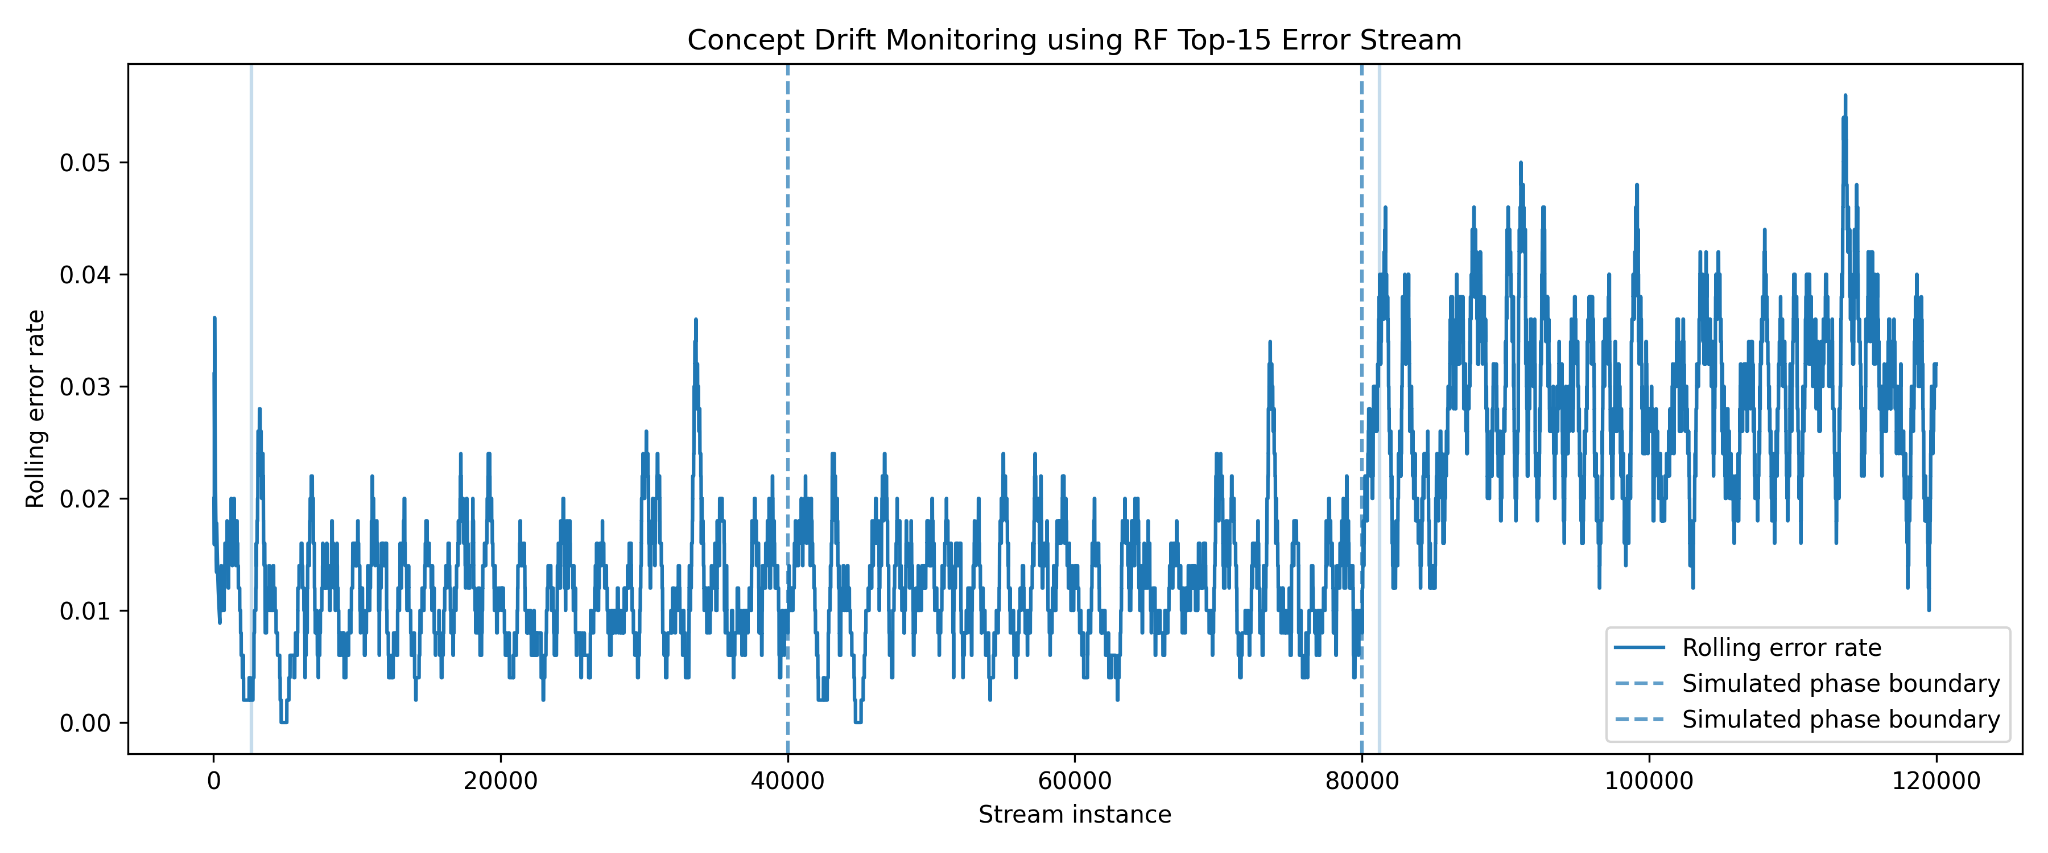
\includegraphics[width=0.78\textwidth]{figures/rf_top15_drift_monitoring.png}
\caption{Concept-drift monitoring using the RF Top-15 prediction-error
stream. The rolling error rate increases after the later phase boundary,
supporting the need for adaptive retraining.}
\label{fig:monitor}
\end{figure}

\subsection{Extended Multiclass Attack Category Evaluation}
\label{sec:multiclass}

Although the main contribution is binary lightweight drift-aware
detection, an extended multiclass experiment was also performed to
evaluate attack-family classification. The original labels were grouped
into BENIGN, DDOS, DOS, MIRAI, SPOOFING, VULNERABILITY\_SCAN, and Other,
where Other aggregates the categories with fewer than 1{,}000 available
records (Reconnaissance, Web/Malware, and Brute Force). A capped
sampling strategy was then applied: each category contributed
$\min(n_c, 20{,}000)$ records, so that the two largest categories
(BENIGN and DDOS) were capped at 20{,}000 while all available records
were retained for every smaller category. This yields
$20{,}000 + 20{,}000 + 19{,}238 + 7{,}693 + 1{,}346 + 1{,}108 + 1{,}094
= 70{,}479$ records. Note that this strategy deliberately preserves the
residual class imbalance rather than equalizing all classes, which is
why accuracy and Macro-F1 diverge by roughly eleven points in
Table~\ref{tab:multiclass}: the larger categories inflate accuracy while
the smaller ones depress the macro average.

Table~\ref{tab:multiclass} shows that full features remain more useful
for detailed attack-family diagnosis than the reduced Top-15 subset.

\begin{table}[!ht]
\centering
\caption{Extended multiclass attack category classification results.}
\label{tab:multiclass}
\small
\resizebox{\textwidth}{!}{%
\begin{tabular}{lccccccc}
\toprule
\textbf{Model} & \textbf{Feat.} & \textbf{Acc.} & \textbf{Macro-F1} &
\textbf{Weighted-F1} & \textbf{Bal. Acc.} & \textbf{MCC} &
\textbf{ROC-AUC} \\
\midrule
RF Full-39            & 39 & 84.85 & 73.56 & 84.25 & 0.6988 & 0.8024 & 0.9720 \\
RF Top-15             & 15 & 81.38 & 70.61 & 80.60 & 0.6723 & 0.7580 & 0.9628 \\
HistGB Top-15         & 15 & 81.48 & 70.18 & 80.72 & 0.6738 & 0.7582 & 0.9662 \\
Extra Trees Top-15    & 15 & 79.80 & 69.52 & 79.56 & 0.7022 & 0.7423 & 0.9604 \\
Decision Tree Top-15  & 15 & 76.61 & 65.52 & 77.31 & 0.6940 & 0.7001 & 0.8708 \\
Logistic Reg.\ Top-15 & 15 & 65.18 & 51.89 & 67.85 & 0.6118 & 0.5648 & 0.9353 \\
Gaussian NB Top-15    & 15 & 53.23 & 40.29 & 51.75 & 0.5623 & 0.4656 & 0.9237 \\
\bottomrule
\end{tabular}}
\end{table}

The multiclass experiment shows that binary intrusion detection and
attack-family diagnosis have different feature requirements. The Top-15
feature set is effective for lightweight binary detection and drift
adaptation, while detailed multiclass diagnosis benefits from richer
feature representation. The lower Macro-F1 relative to accuracy also
confirms that minority attack families remain the harder case, which is
consistent with reports elsewhere in the IoT IDS literature
\cite{mishra2024,shanmugam2025}.

\subsection{Cybersecurity Application Implications}

The proposed framework is suitable as a first-stage gateway-level IoT
cyber monitoring component. Its Top-15 feature subset avoids payload
inspection and relies on flow-level statistical attributes. This is
useful when payload access is unavailable because of encryption, privacy
restrictions, or resource limitations. The drift-triggered retraining
mechanism also provides an operational response to changing traffic
conditions. Instead of assuming that an IDS model remains valid
indefinitely, L-CDAIDS monitors prediction-error behavior and updates
the model when drift is detected.

The reduction in Phase-3 false positives is particularly important. The
static Top-15 model produced a Phase-3 FPR of 0.2899, whereas the
proposed drift-triggered model reduced it to 0.0075. In operational
terms, this means fewer benign flows are incorrectly escalated as
malicious after distributional change. Section~\ref{sec:robustness}
strengthens this point: the static configuration's false-alarm behavior
is not merely elevated on average but intermittently catastrophic,
whereas the retrained model's Phase-3 FPR never exceeded 0.8\% in any
replication of any configuration tested.

\subsection{Consolidated Experimental Settings}
\label{sec:settings}

The paper reports results from several distinct experimental protocols,
distinguished mainly by Random Forest configuration and data-partition
scheme (Section~\ref{sec:protocol} already calls out the two most easily
confused ones). Table~\ref{tab:settings} consolidates, for every result
table, the exact forest configuration, split protocol, and script name,
so that any result can be traced to its code without cross-referencing
prose. All scripts are released with the repository (Data and Code
Availability).

\begin{longtable}{p{3.1cm} p{3.6cm} p{4.1cm} p{3.6cm}}
\caption{Consolidated experimental settings: Random Forest configuration,
data-partition protocol, and script, for every result table in the paper.}
\label{tab:settings} \\
\toprule
\textbf{Result} & \textbf{Forest configuration} & \textbf{Split protocol} &
\textbf{Script} \\
\midrule
\endfirsthead
\multicolumn{4}{c}{\tablename\ \thetable{} -- continued} \\
\toprule
\textbf{Result} & \textbf{Forest configuration} & \textbf{Split protocol} &
\textbf{Script} \\
\midrule
\endhead
\bottomrule
\endfoot
Tables~\ref{tab:rf-feature}, \ref{tab:classifiers} (static binary baseline) &
100 trees, max\_depth 20, unweighted, random\_state 42 &
Single fixed stratified 80:20 split, random\_state 42 &
\texttt{classifier\_comparison\_fixed.py} \\
5-fold CV (Section~\ref{sec:cv}) &
100 trees, max\_depth 20, unweighted, random\_state 42 (same for every fold) &
\texttt{StratifiedKFold}, 5 folds, random\_state 42; the global Top-15 list
is reused in every fold, not re-ranked within it &
\texttt{cross\_validation\_tables\_3\_4.py} \\
Tables~5, 6, 8, \ref{tab:cost}, Figs.~2--4, drift/retrain events &
50 trees, \texttt{class\_weight="balanced"} &
One fixed stratified 80:20 split (random\_state 42) reused for all three
seeds; only the forest's own random\_state varies (= seed) &
\texttt{notebooks/concept\_drift\_three\_seed\_FULL\_recovered.ipynb} \\
Table~\ref{tab:fifteen} (fifteen-seed robustness) &
100 trees, max\_depth 20, unweighted, random\_state 42 (fixed) &
Fresh independent stratified 80:20 split per seed (random\_state = seed) &
\texttt{three\_seed\_concept\_drift.py} \\
Table~\ref{tab:disentangle} (seed-vs-split disentangling) &
50 trees, \texttt{class\_weight="balanced"}, random\_state = seed &
Fresh independent stratified 80:20 split per seed (random\_state = seed);
both split and forest randomness vary together &
\texttt{disentangle\_seed\_vs\_split.py} \\
ARF comparison (Section~\ref{sec:arf}, ARF rows of Table~\ref{tab:cost}) &
\texttt{river} \texttt{ARFClassifier}, 10 models &
Same fixed 80:20 split as Tables 5--6 (random\_state 42); RF-side rows of
Table~\ref{tab:cost} reused from the recovered notebook above &
\texttt{arf\_baseline.py} \\
Table~\ref{tab:fullaffine} (corpus covariate shift) &
50 trees, \texttt{class\_weight="balanced"} &
674{,}994-flow quota pool (Table~\ref{tab:quota}); fresh per-seed
train/stream draw from that pool &
\texttt{drift\_experiment\_fulldata.py --stream affine} \\
Table~\ref{tab:family} (corpus family holdout) &
50 trees, \texttt{class\_weight="balanced"} &
Same quota pool; per-seed known/novel stream draw (Table~\ref{tab:phasequota}) &
\texttt{drift\_experiment\_fulldata.py --stream family} \\
Table~\ref{tab:configrobust} (100-tree corpus robustness check) &
100 trees, max\_depth 20, unweighted &
Identical quota pool and protocol as Tables~\ref{tab:fullaffine},
\ref{tab:family}; only the forest constructor changed &
\texttt{drift\_experiment\_fulldata.py} (RF constructor swapped) \\
Table~\ref{tab:sweep} (mixing-ratio sweep) &
50 trees, \texttt{class\_weight="balanced"} &
Same quota pool; \texttt{--novel-frac} 0.25/0.50/0.75, seed 42 &
\texttt{drift\_experiment\_fulldata.py --novel-frac} \\
Table~\ref{tab:chrono} (chronological evaluation) &
50 trees, \texttt{class\_weight="balanced"} (reuses the drift-experiment
helpers) &
File-order split (train on files 1--44, stream on 45--63) vs. a random
split of identical size &
\texttt{chrono\_experiment.py} \\
Multiclass tables (Section~\ref{sec:multiclass}) &
100 trees, max\_depth 20, unweighted, random\_state 42 &
Single fixed stratified 80:20 split, random\_state 42 &
\texttt{multiclass\_attack\_classification\_fixed.py} \\
Table~\ref{tab:pi15} (Raspberry Pi, \texttt{tab:fifteen} protocol) &
100 trees, max\_depth 20, unweighted, random\_state 42 (fixed) &
Fresh independent stratified 80:20 split per seed, run on a Raspberry
Pi~4 rather than the workstation &
\texttt{pi\_benchmark\_lcdaids.py} \\
Table~\ref{tab:picost} (Raspberry Pi, \texttt{tab:cost} protocol) &
50 trees, \texttt{class\_weight="balanced"} &
One fixed 80:20 split reused across seeds, run on a Raspberry Pi~4 &
\texttt{pi\_benchmark\_tabcost.py} \\
\end{longtable}

%---------------------------------------------------------------------
\FloatBarrier
\section{Limitations and Future Work}
\label{sec:limitations}

This study has six limitations. First, neither drift regime is a naturally
chronological IoT traffic stream. The covariate-shift regime is an injected
perturbation, and while the attack-family holdout of
Section~\ref{sec:familystream} is real concept drift rather than a scaling
artefact, the point at which new families appear is still chosen by the
experimenter rather than observed in time. This is a limitation of the dataset
rather than a step the study declined to take:
Section~\ref{sec:chrono} shows that the CICIoT2023 feature release carries no
timestamp field and that its 63 capture files are statistically homogeneous, so
a file-order train-on-earlier, test-on-later split was measured to be
equivalent to a random split to within seed noise
($\Delta$F$_1 = 0.00018$). Establishing temporal drift in IoT traffic requires
a release that retains capture timestamps, such as the Zeek connection logs of
IoT-23 \cite{garcia2020iot23}, whose flow schema differs from CICIoT2023 and
which therefore cannot be used to evaluate the present Top-15 subset without
first deriving a fresh feature ranking. That is cross-dataset work rather than
an extension of this evaluation. Second, the entire pipeline assumes
ground-truth labels arrive immediately after each prediction
(Section~\ref{sec:drift}), and this assumption is not confined to
retraining: ADWIN's drift detections, and therefore the point at which
retraining can even be triggered, are only as timely as the labels
feeding the error stream. In production, labels typically come from
delayed analyst review or confirmed incident reports rather than an
oracle, so both detection and retraining would lag by however long
labeling takes, and the recent-window retraining strategy additionally
assumes access to labeled samples once they do arrive. Semi-supervised
or delayed-label variants --- for instance, monitoring a proxy signal
such as prediction-confidence drift while awaiting labels, or
quantifying how much the detection lag Section~\ref{sec:drift} depends
on grows as labeling delay increases --- are an important next step,
and the degree to which this assumption weakens the paper's
conclusions scales directly with how quickly a given deployment can
obtain ground truth.
Third, the main contribution is optimized for binary intrusion
detection; multiclass attack-family classification remains more
difficult, especially for minority categories. Relatedly, the family-holdout
result quantifies how poorly a static detector generalises to unseen families
but does not identify \emph{which} families are hardest; a per-family recall
breakdown would sharpen the operational guidance and is a natural extension. Fourth, detection-quality
evaluation throughout the paper is conducted in a workstation environment;
Section~\ref{sec:robustness} and Section~\ref{sec:arf} report that the
accuracy figures reproduce on a Raspberry~Pi~4 and additionally quantify
real CPU, memory, and latency costs there, but the ARF baseline and the
full 34.3M-flow corpus-scale experiments of
Sections~\ref{sec:fullcorpus}--\ref{sec:family} were not re-run on
constrained hardware, so gateway-class cost figures for those remain an
open question. Fifth, the study uses CICIoT2023 as the primary dataset, and
cross-dataset validation remains necessary.

Sixth, the binary detector is trained and evaluated on a class-balanced
(50:50 benign/attack) sample. Precision, false-positive rate, and other
operating-point metrics reported here are specific to this balanced
setting and will differ under the much lower attack prevalence typical
of real IoT deployments; recalibration or threshold adjustment would
likely be needed before production use. This caveat applies equally to
the comparison baselines and does not affect the relative ordering of
the models, but it does affect the absolute numbers a deployment should
expect.

Future work will address these limitations by evaluating L-CDAIDS on
timestamped traffic traces --- IoT-23 \cite{garcia2020iot23} is the most
suitable candidate, since its Zeek connection logs retain per-flow capture
times across twenty-three scenarios recorded in 2018--2019 --- and on
additional datasets such as Bot-IoT, N-BaIoT, ToN-IoT, and Edge-IIoTset
\cite{koroniotis2019,meidan2018,moustafa2021,ferrag2022}. Because these
releases do not share the CICIoT2023 feature schema, such an evaluation
requires re-deriving the importance ranking on each schema and asks a
different question: whether the \emph{method} of ranking-then-reducing
transfers, rather than whether this particular fifteen-feature subset does. Future
experiments will also compare ADWIN with DDM, EDDM, and Page-Hinkley
drift detectors, extend the Adaptive Random Forest comparison of
Section~\ref{sec:arf} to larger ensembles and to other streaming
learners on gateway-class hardware (the ARF baseline itself was not
re-measured on the Raspberry Pi here, for the reasons given in
Section~\ref{sec:arf}), and evaluate semi-supervised or delayed-label
retraining. Federated drift-aware training may also be explored for
privacy-preserving collaboration among IoT gateways.

%---------------------------------------------------------------------
\section{Conclusion}
\label{sec:conclusion}

This paper presented L-CDAIDS, a lightweight concept-drift-aware IDS
framework for resource-constrained IoT networks. The
framework first constructs a balanced and feature-optimized Random
Forest IDS using CICIoT2023. The Top-15 feature subset achieved 98.85\%
accuracy and 98.84\% F1-score in the static balanced binary setting,
nearly matching the full 39-feature model while reducing feature
dimensionality by 61.54\%; five-fold cross-validation confirms this
baseline is stable to within $\pm 0.0002$ accuracy.

The main contribution extends the static lightweight model with
concept-drift awareness. A controlled three-phase, 120{,}000-sample
evolving stream was constructed to test robustness under changing IoT
traffic. Across three seeds, the drift-triggered RF Top-15 model
achieved 0.9857 accuracy, 0.9856 F1-score, and 0.9716 MCC,
outperforming both the static full-feature and static lightweight
baselines in overall mean performance. The strongest evidence appeared
in Phase~3, where the static Top-15 model dropped to 0.8809 F1-score and
0.7376 MCC, whereas the proposed drift-triggered model maintained 0.9832
F1-score and 0.9668 MCC.

A dedicated sensitivity analysis further established that this
degradation is a property of the compact, class-weight-balanced forest
configuration rather than of any particular data partition, and that
drift-triggered retraining removes the resulting false-alarm failure
mode across every configuration tested. Against the Adaptive Random
Forest baseline, L-CDAIDS achieved statistically indistinguishable
detection quality while processing the stream $25.3\times$ faster and
building its initial model $9.7\times$ faster, indicating that the
robustness of a streaming ensemble can be obtained at close to static
lightweight cost.

The framework was then re-evaluated on the complete 34{,}298{,}828-flow corpus
under a stricter regime in which entire attack families were withheld from
training and introduced mid-stream. This produced the study's most
operationally significant finding: the static lightweight detector operates at
unchanged recall on the families it was trained on (0.986) and a false-positive
rate of one in a thousand, while recovering only 1.3\% of withheld web/malware
and brute-force traffic. Nothing an operator can observe indicates that anything
has changed: the failure is silent, which makes it more dangerous than the
noisy degradation seen under covariate shift. Drift-triggered retraining lifts
withheld-family recall from 0.013 to 0.522 --- a substantial but only partial
recovery, since roughly 48\% of withheld-family attacks are still missed, now
at a 7.4\% false-positive rate rather than the near-zero rate of the undrifted
phase. An adaptive-normalisation baseline confirms that the loss cannot be
recovered by rescaling inputs ---
under real concept drift renormalisation drives the false-positive rate to 0.97
and Matthews correlation to 0.06. A further finding qualifies the
feature-reduction claim itself: on reconnaissance the full 39-feature detector
recovers 0.336 of withheld attacks against 0.235 for the Top-15 subset, despite
the two being statistically indistinguishable on static held-out data. Taken
together, these results show that feature reduction alone is not enough under
evolving traffic, that the adaptation mechanism is doing work no input-side
correction can substitute for, and that ADWIN-based drift detection with
recent-window Random Forest retraining maintains robust --- and, critically,
predictable --- lightweight IDS performance.

Two boundary conditions are reported alongside these gains. A file-order
train-on-earlier, test-on-later split of the corpus was measured to be
equivalent to a random split to within seed noise, because the CICIoT2023
feature release carries no timestamp and its capture files are statistically
homogeneous; temporal drift is not demonstrable from this release, and the
synthetic regimes used here are not a convenience but the only option it
supports. In that undrifted setting the adaptation mechanism costs 0.001 in
F$_1$ and $4.2\times$ the streaming time --- the price of carrying the
mechanism when there is nothing to adapt to, set against recoveries of 0.16 in
F$_1$ under covariate shift and roughly one to two orders of magnitude (25- to
forty-fold, depending on the static forest's configuration,
Section~\ref{sec:robustness}) in withheld-family recall. That asymmetry,
rather than any single accuracy figure, is the case for deploying
drift-triggered retraining on constrained IoT gateways.

%---------------------------------------------------------------------
\section*{Statements and Declarations}

\subsection*{Funding}
The author did not receive support from any organization for the
submitted work.

\subsection*{Competing Interests}
The author declares no known competing financial or
non-financial interests that are directly or indirectly related to the
work submitted for publication.

\subsection*{Author Contributions}
Amiya Kumar Sahu is the sole author of this work and is responsible for
conceptualization, methodology, software implementation, data curation,
validation, formal analysis, investigation, visualization, supervision,
and writing (original draft, review, and editing).

\subsection*{Acknowledgements}
During the preparation of this work, the author used Claude (Anthropic;
Claude Opus 5 and Claude Sonnet 5, accessed August--September 2026) to
assist with literature search and synthesis, implementation and execution
of the experiments reported in Sections~\ref{sec:results}
and~\ref{sec:limitations}, statistical analysis of the results, and
drafting and revision of the manuscript text. After using this tool, the
author reviewed, verified, and edited all content, experimental design
choices, and conclusions, and takes full responsibility for the content
of this publication.

\subsection*{Data and Code Availability}
The CICIoT2023 dataset used in this study is publicly available from the
Canadian Institute for Cybersecurity, University of New Brunswick.
Because of dataset size and redistribution considerations, the raw
CICIoT2023 files are not redistributed with this manuscript. The source
code, preprocessing scripts, concept-drift notebooks --- including the
complete three-seed, phase-wise, and drift-triggered-retraining
experiment behind Tables~\ref{tab:overall}, \ref{tab:phasewise} and
\ref{tab:events}, the scripts for the cross-validation and
sensitivity analyses of Tables~\ref{tab:cv}, \ref{tab:disentangle} and
\ref{tab:fifteen}, and the full-corpus sampler and two-regime drift experiment
behind Tables~\ref{tab:corpus}, \ref{tab:fullaffine} and \ref{tab:family} --- together with result tables, figures, and
reproducibility resources are publicly available at
\url{https://github.com/idofamiya/lightweight-balanced-iot-ids}.

\subsection*{Ethics Approval}
Not applicable. This study does not involve human participants, animals,
or clinical data.

\subsection*{Consent to Participate}
Not applicable.

\subsection*{Consent for Publication}
Not applicable.

%---------------------------------------------------------------------
\clearpage
\bibliographystyle{unsrt}
\bibliography{references}

\end{document}
